

\chapter{Diseño e implementación} % Main chapter title

\label{Chapter3} % Change X to a consecutive number; for referencing this chapter elsewhere, use \ref{ChapterX}



En este capítulo se presentan los detalles del diseño de los nodos sensores y actuadores que conforman el trabajo, como así también los del software seleccionado.

\section{Arquitectura de la solución}
\label{sec:Arquitectura de la solución}

%Como se observa en la figura \ref{fig:blockdiagram}, el invernadero inteligente está compuesto por un conjunto de subsistemas encargados de las diferentes funciones de medición y control de variables, una aplicación central y un sistema que permita el acceso remoto de forma segura.

Para la implementación del prototipo propuesto en el trabajo se requirió la construcción de diferentes subsistemas encargados de las múltiples funciones dentro del invernadero inteligente. Cada uno de ellos opera en forma independiente del resto y se comunican con una aplicación central mediante una red inalámbrica. 
Para garantizar el acceso de los usuarios desde Internet se desarrolló una interfaz de acceso remoto.





\subsection{Componentes del sistema}
\label{Componentes del sistema}

En la figura \ref{fig:blockdiagram} se observa el diagrama en bloques de la arquitectura diseñada, que está compuesta por los siguientes elementos: 

\begin{itemize}
\item Sistema de monitoreo y control de clima, formado por dos módulos:
\begin{itemize}
\item Sensores de temperatura y humedad con sus correspondientes microcontroladores.
\item Unidad de control de temperatura y humedad comprendida por un microcontrolador, relé y ventiladores. 
\end{itemize}
Los sensores miden la temperatura y humedad ambiente en el invernadero y envían estos valores a la aplicación central por medio del microcontrolador. De acuerdo con los datos recibidos, la aplicación determina si es necesario emitir una señal para que la unidad de control encienda los ventiladores.



\item Sistema de control de riego, dividido en dos partes:
\begin{itemize}
\item Conjunto de sensores de humedad de suelo con sus respectivos microcontroladores.
\item Unidad de control de riego constituida por un microcontrolador, relés, bomba de agua y válvulas.
\end{itemize}

Los sensores envían las mediciones a la aplicación central que se encarga de procesarlas. En caso de ser necesario, se disparan las señales de encendido a través de la unidad de control. Primero se activa la válvula que corresponda y luego se enciende la bomba de agua para comenzar el riego. El orden de estas actividades es importante para evitar daños en la bomba o las cañerías.

\item Aplicación central. Constituye el cerebro del invernadero y es la encargada de almacenar los parámetros de configuración de los diversos sensores y actuadores, procesar los mensajes recibidos, disparar acciones y alertas y visualizar el estado general.

\item Sistema de acceso remoto. Permite a los usuarios obtener reportes del sistema en forma segura desde Internet.   
\end{itemize}



\begin{figure}[h]
	\centering
	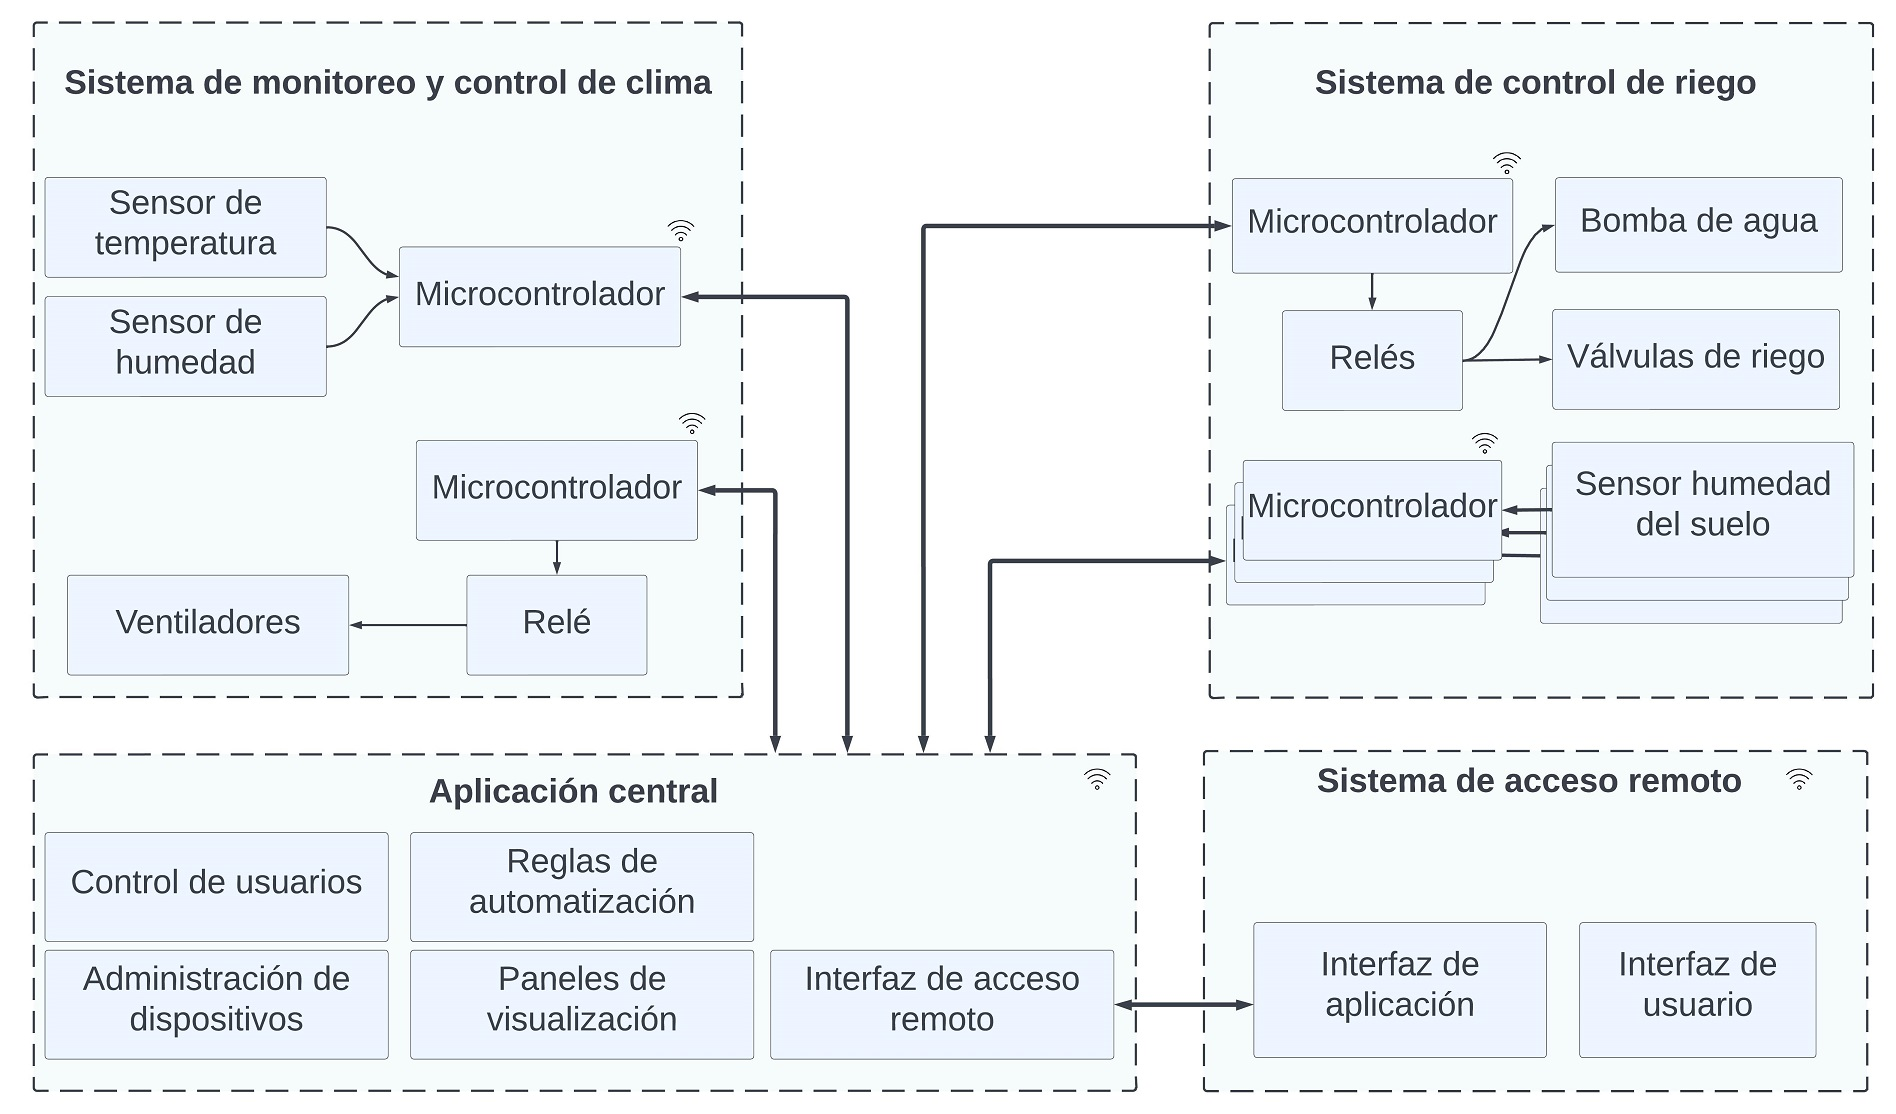
\includegraphics[width=1.0\textwidth]{./Figures/blockdiagram4.jpg}
	\caption[Arquitectura del sistema.]{Arquitectura del sistema.}
	\label{fig:blockdiagram}

\end{figure}


\subsection{Protocolos de comunicación}
\label{Protocolos de comunicación}
%\textit{Aquí se describe cómo se comunican los sistemas con la aplicación central y los protocolos usados en cada caso.}

%En la selección del software de la aplicación central se contempló la compatibilidad con múltiples protocolos de comunicación. Sin embargo limitaciones de configuración específicas, tal como el tiempo de retención de los mensajes en las colas de MQTT, forzaron el utilizar diferentes protocolos dependiendo del módulo en cuestión. Otro factor condicionante, como se detalla en la sección \ref{sec:Ciberseguridad del sistema}, fue el carecer de una CA que emita certificados que todos los componentes puedan confiar.

En esta sección se describe cómo se comunican los sistemas con la aplicación central y los protocolos usados en cada caso. En la figura \ref{fig:blockprotos} se aprecia un esquema simplificado que ilustra dichas interacciones.

Si bien los módulos de hardware y el software soportan una gran variedad de protocolos,  se implementó MQTT en la mayoría de los casos conforme a los requerimientos. En algunas situaciones donde esto no fue técnicamente posible, se utilizó HTTP. Adicionalmente, para garantizar la seguridad de las comunicaciones, se incorporó un certificado autofirmado TLS en el servidor.

\begin{figure}[h]
	\centering
	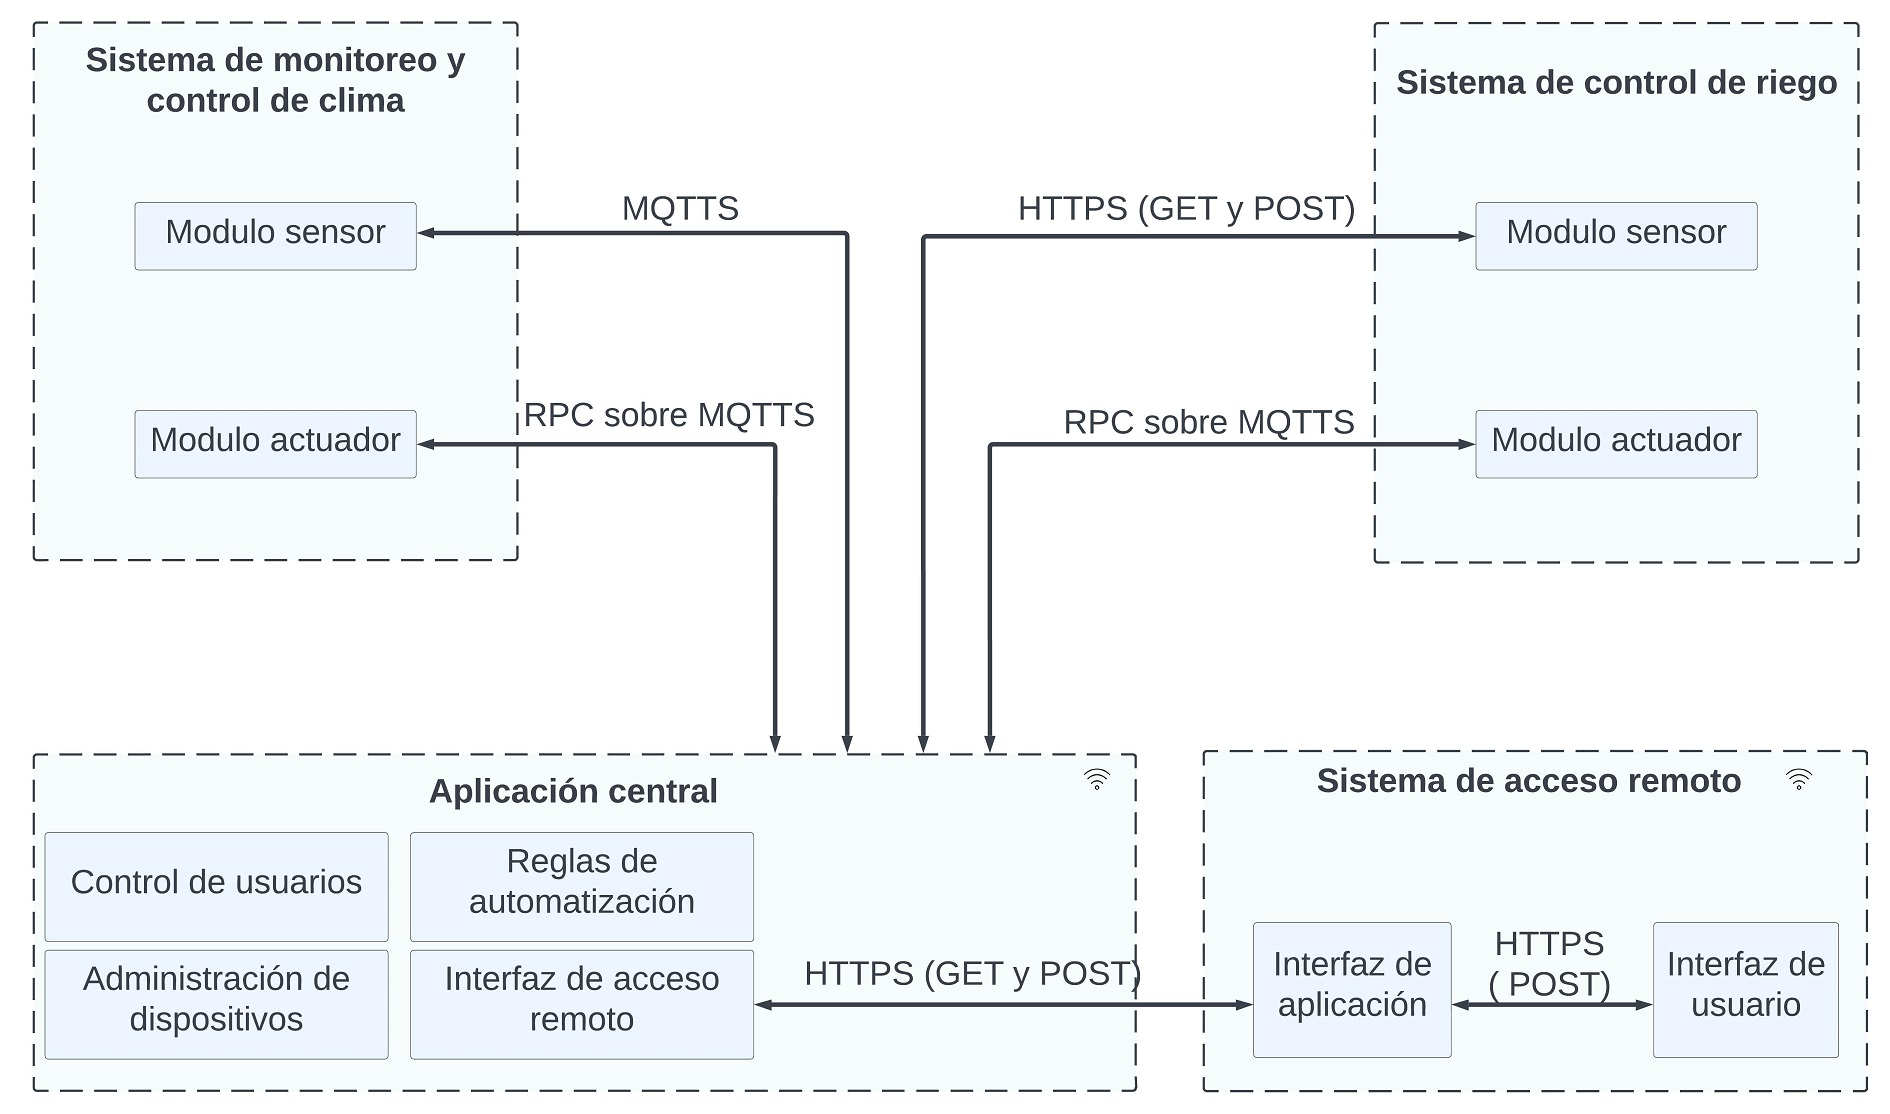
\includegraphics[width=1.0\textwidth]{./Figures/blockproto2.jpg}
	\caption[Protocolos de comunicación entre módulos.]{Protocolos de comunicación entre módulos.}
	\label{fig:blockprotos}
\end{figure}


\pagebreak
Las interacciones principales entre los bloques componentes son:
 
 \begin{itemize}
	\item Sistema de monitoreo y control de clima: las comunicaciones se realizan exclusivamente con aplicación central.
	El módulo sensor envía las mediciones realizadas por medio de MQTT y en caso de requerir una acción, la aplicación central comanda el encendido de los ventiladores por medio de un mensaje enviado por RPC \citep{rfc1057} sobre MQTT.
	
	\item Sistema de control de riego: las comunicaciones se realizan con la aplicación central de manera bidireccional.
	El módulo sensor efectúa dos conexiones, una para el envío de las mediciones y otra para recibir valores de atributos tales como la duración del tiempo de riego. Debido a limitaciones en la configuración de la persistencia de los mensajes en las colas de MQTT, se optó por utilizar llamadas HTTP (GET y POST) para realizarlas.
	Al igual que en el control de clima, la aplicación central inicia el riego por medio de mensajes RCP sobre MQTT hacia el controlador de la bomba y de las válvulas.
	
	\item Sistema de acceso remoto: la interfaz se comunica con la aplicación por medio de pedidos HTTP GET y POST para consultar el reporte de estado de los diferentes componentes. A continuación este se envía hacia la interfaz de usuario por medio de una solicitud HTTP POST.
 
 
 
 
 \end{itemize}






\section{Detalle de los módulos de hardware}
\label{sec:Módulos de hardware}
En esta sección se describen en detalle los esquemas de conexión de los distintos módulos y las consideraciones de diseño y construcción empleadas. 

\subsection{Módulos sensores de humedad del suelo}
\label{Módulos sensores de humedad del suelo}


En el proyecto se desarrollaron dos configuraciones diferentes de módulos para medir la humedad del suelo en macetas de diverso tipo y tamaño. Ambas opciones utilizan el microcontrolador ESP8266 pero incorporan distinta cantidad de sensores. En la figura \ref{fig:soilschem1} se muestra el esquema de conexión para la versión simple (con un único sensor) y en la figura \ref{fig:soilschem2} se ilustra la configuración doble.

Si bien en el prototipo los sensores se conectaron a una fuente de alimentación, la configuración y conexión del sistema está optimizada para el uso de baterías. Esto se debe a que las sondas pueden estar desplegadas en múltiples ubicaciones dentro del invernadero y no siempre es posible conectarlas a la red eléctrica. 

El ahorro de energía necesario para permitir el uso de  baterías se logra a través de ciclos de apagado en los períodos donde no se realizan lecturas. A este mecanismo se lo que conoce como \textit{deep sleep} y una vez que el microcontrolador se encuentra en este estado se requiere un pulso eléctrico en el pin de \textit{reset} para que retorne al modo activo. 
Para habilitar la reactivación se interconectaron los pines D0 (GPIO16) y RST del chip ESP8266. Se logra así una reducción del consumo de energía a valores muy pequeños que rondan los 0,3 mA durante el período de inactividad.




\begin{figure}[!h]
     \centering
     \begin{subfigure}[b]{0.45\textwidth}
		\centering
		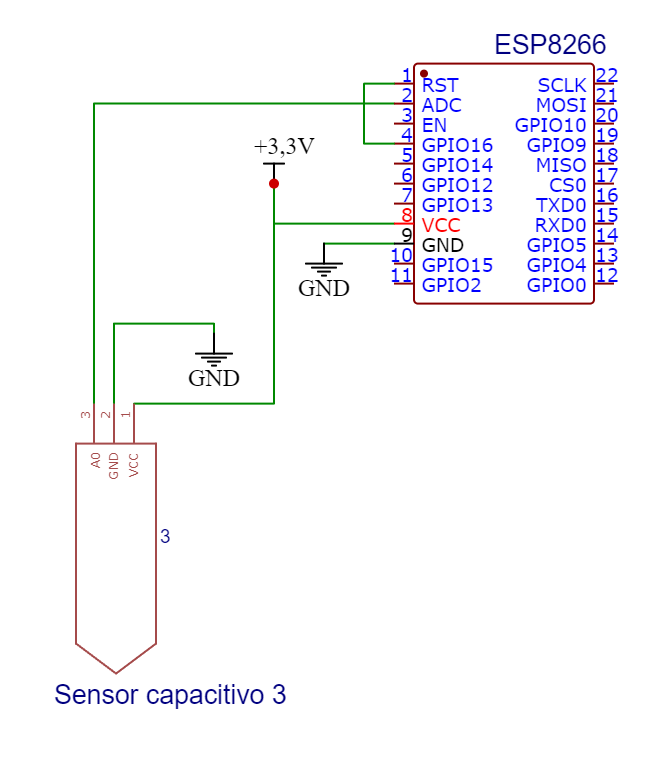
\includegraphics[width=0.9\textwidth]{./Figures/soil_schem_simple.png}
		\caption[Módulo sensor simple]{Módulo sensor simple.}
		\label{fig:soilschem1}
     \end{subfigure}
     \hfill
     \begin{subfigure}[b]{0.45\textwidth}
	\centering
		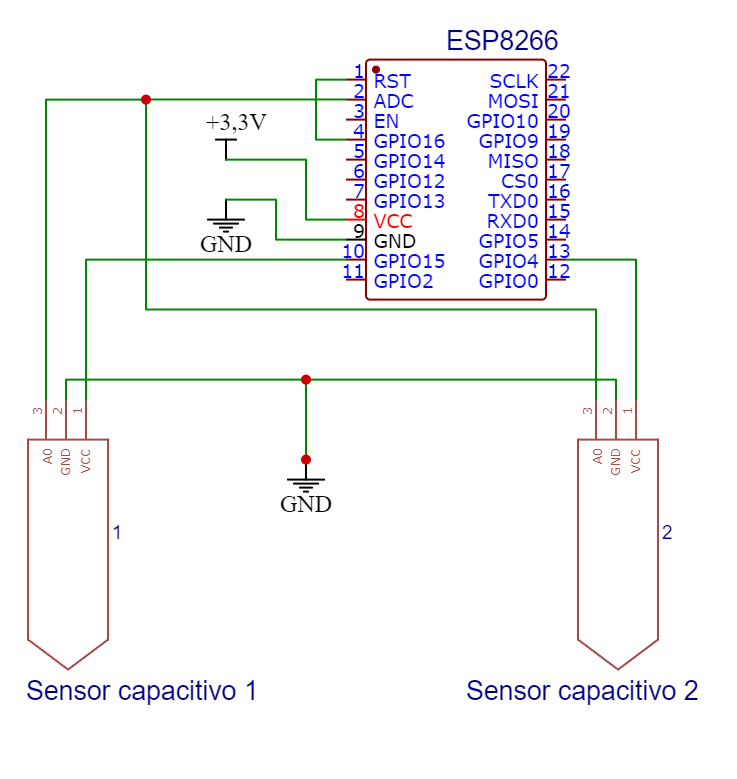
\includegraphics[width=1\textwidth]{./Figures/soil_schem_doble.png}
		\caption[Módulo sensor doble]{Módulo sensor doble.}
		\label{fig:soilschem2}
     \end{subfigure}
     \hfill
        \caption[Esquema de conexión de módulos sensores de humedad del suelo]{Esquema de conexión de módulos sensores de humedad del suelo.}	\label{fig:soilschem}
\end{figure}
%\begin{figure}[!h]
%	\centering
%	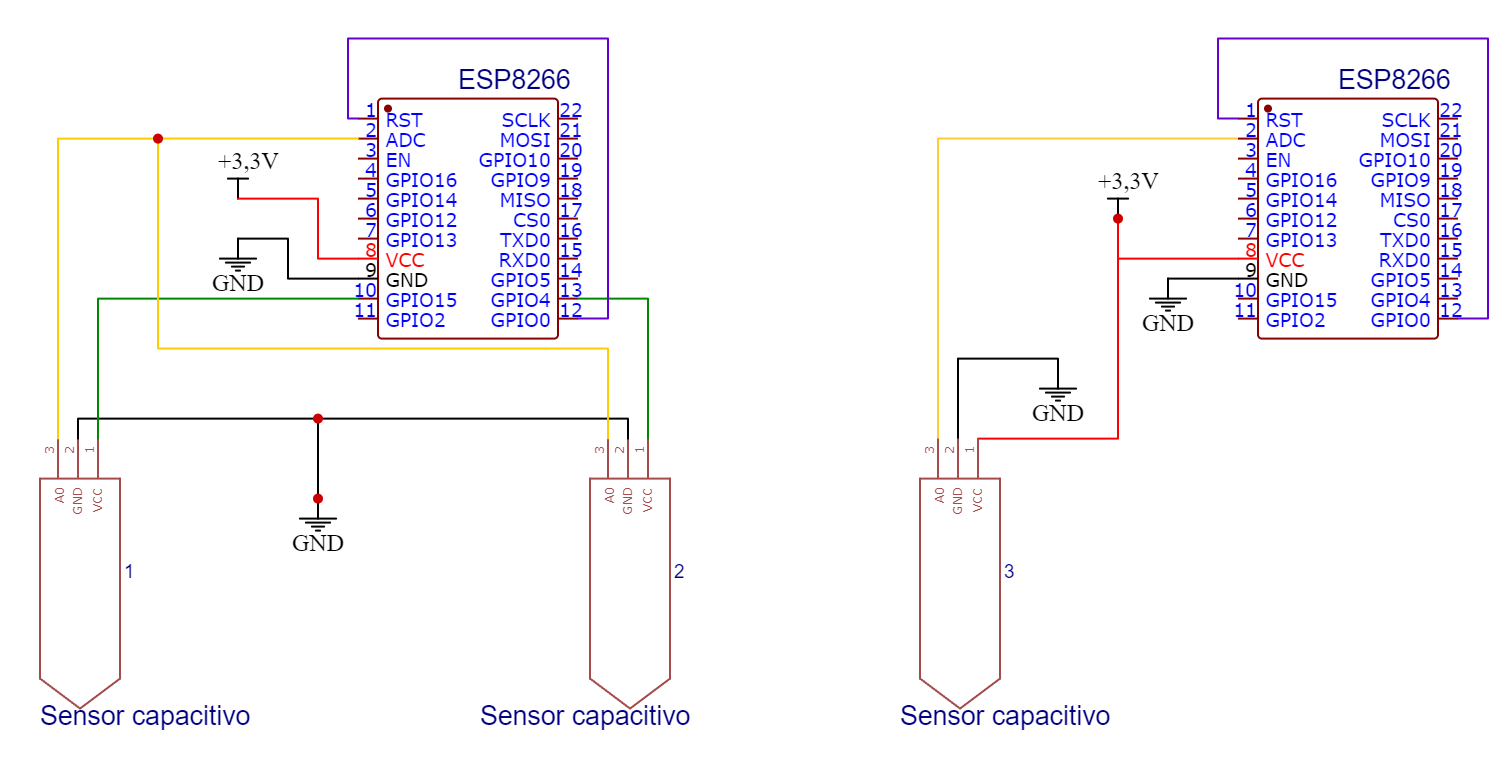
\includegraphics[width=1\textwidth]{./Figures/soil_schematic2.png}
%	\caption[Conexión del sensor de humedad del suelo]{Conexión del sensor de humedad del suelo.}
%	\label{fig:soilschem}
%\end{figure}

La integración de los componentes de los sensores se  realizó en forma manual por medio de placas de circuitos impresos (PCB) experimentales. En las figuras \ref{fig:soil1} y \ref{fig:soil2} se muestran los componentes empleados y un módulo ensamblado.

Dado que los sensores están expuestos a salpicaduras, se los recubrió con tubos adhesivos termocontraíbles que, al aplicarles calor, generan una protección a prueba de agua. Para el resguardo del chip ESP8266 se utilizó una caja de polipropileno transparente sellada. En las figuras \ref{fig:soil3} y \ref{fig:soil4} se muestran los componentes y sus protecciones. 

\begin{figure}[!h]
     \centering
     \begin{subfigure}[b]{0.45\textwidth}
		\centering
		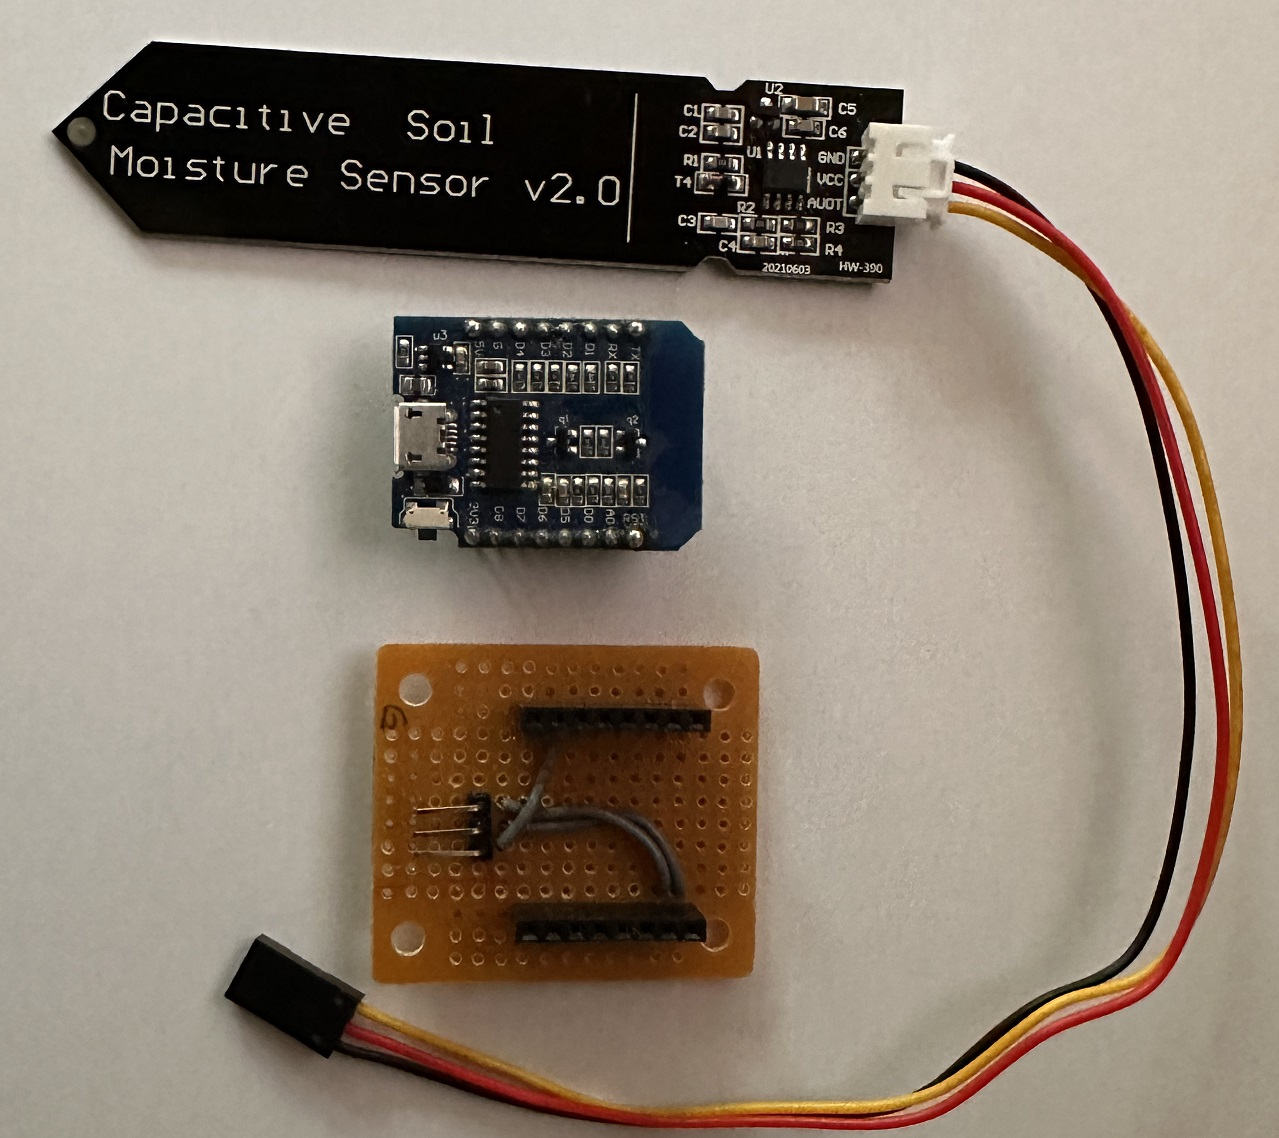
\includegraphics[width=0.80\textwidth]{./Figures/soil1.jpeg}
		\caption[Módulo con un sensor de humedad del suelo]{Módulo con un sensor de humedad del suelo.}
		\label{fig:soil1}
     \end{subfigure}
     \hfill
     \begin{subfigure}[b]{0.45\textwidth}
	\centering
		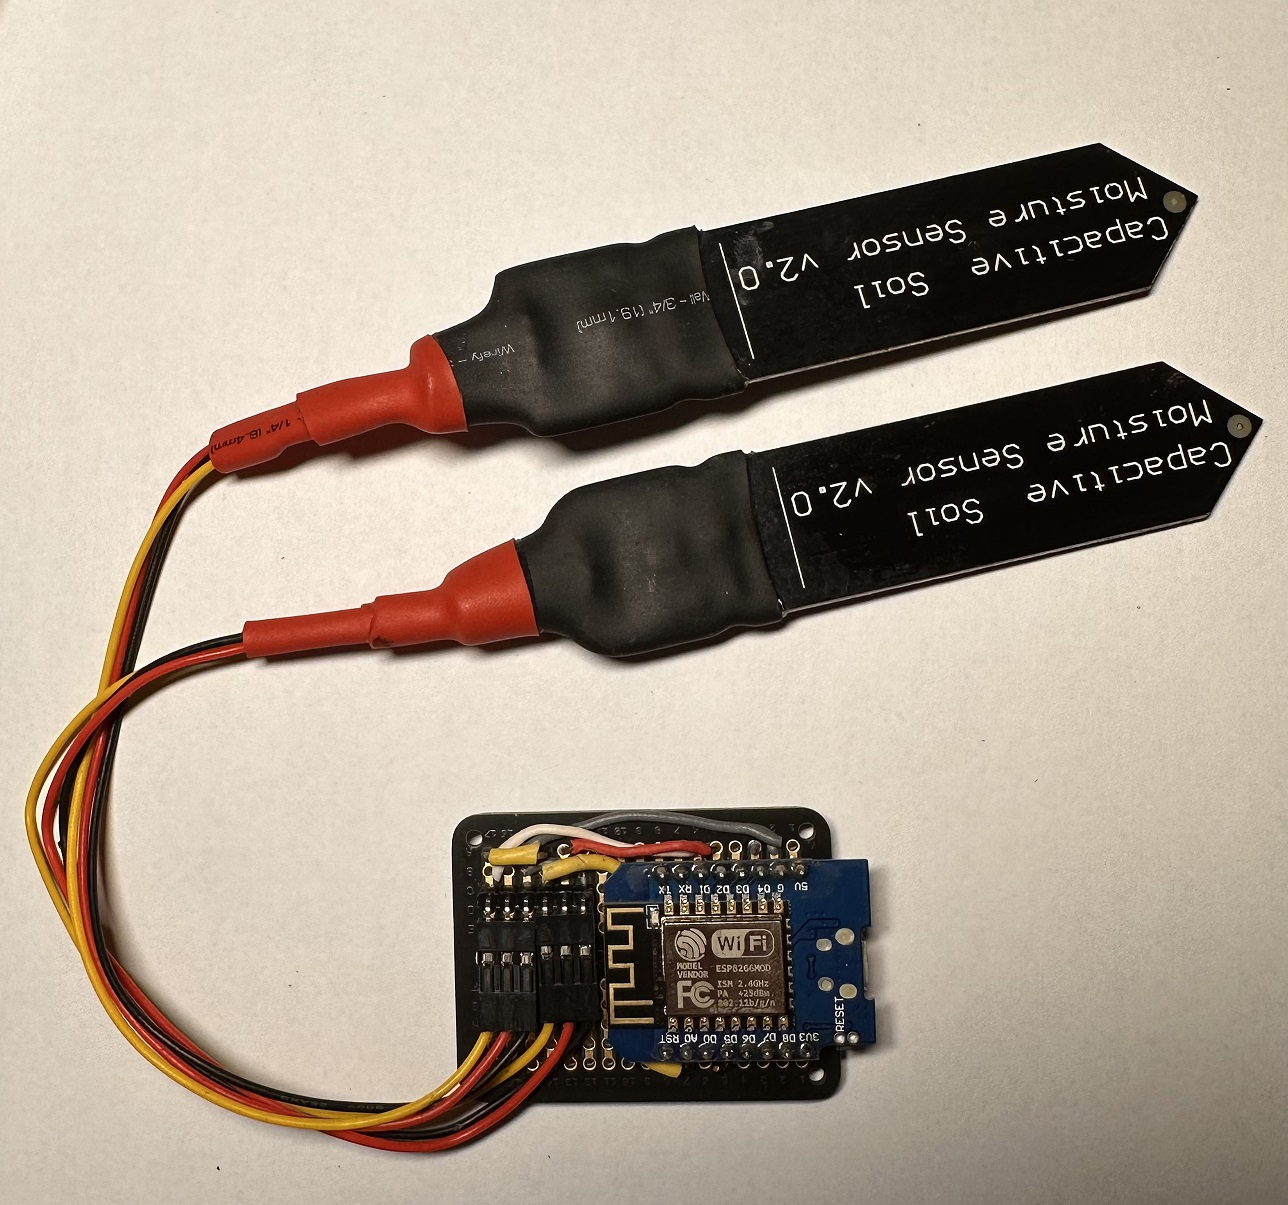
\includegraphics[width=0.80\textwidth]{./Figures/soil2.jpeg}
		\caption[Módulo con dos sensores de humedad del suelo]{Módulo con dos sensores de humedad del suelo.}
		\label{fig:soil2}
     \end{subfigure}
      \begin{subfigure}[b]{0.45\textwidth}
	\centering
		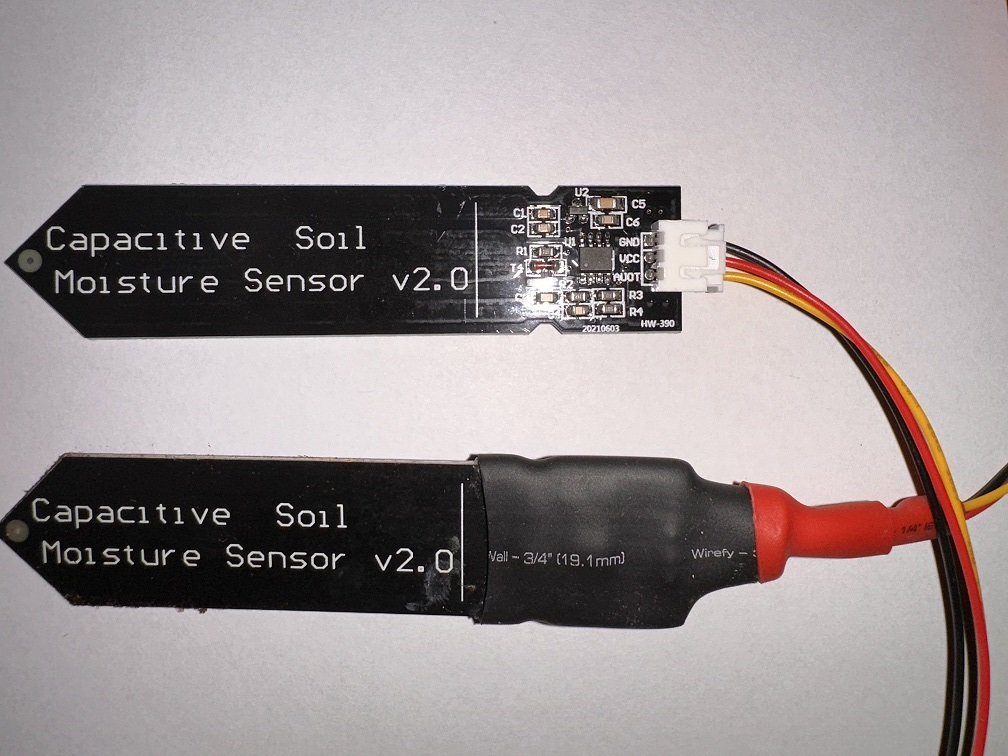
\includegraphics[width=0.80\textwidth]{./Figures/soil_compare.jpg}
		\caption[Detalle de protección de circuitos en los sensores]{Detalle de protección de circuitos en los sensores.}
		\label{fig:soil3}
     \end{subfigure}	
			\begin{subfigure}[b]{0.45\textwidth}
	\centering
		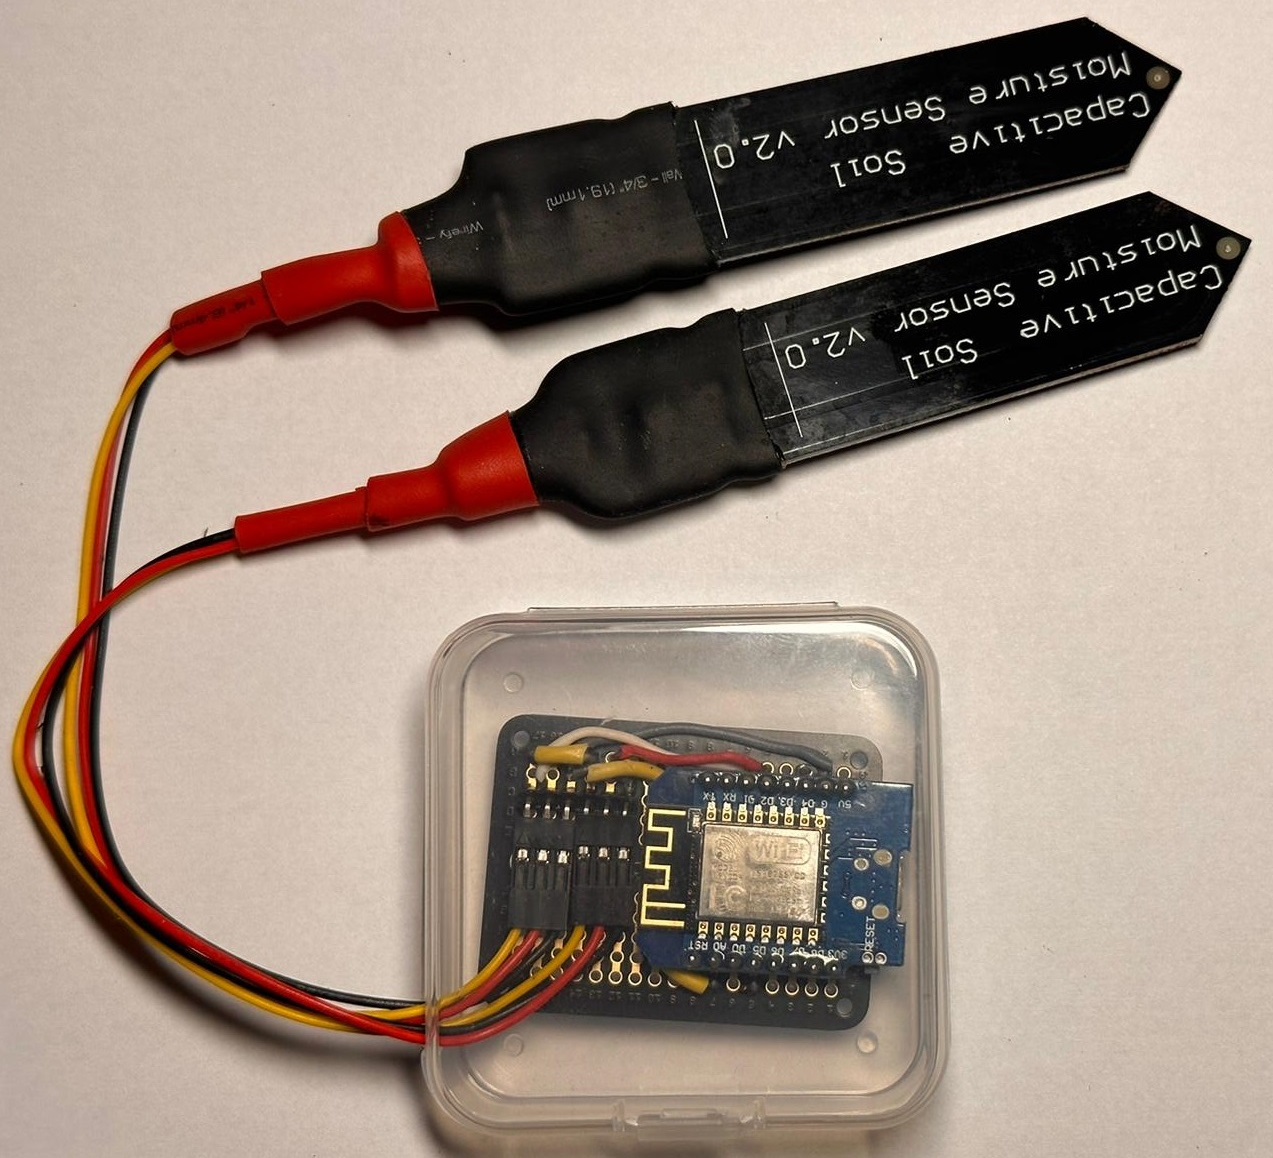
\includegraphics[width=0.80\textwidth]{./Figures/soil3.jpg}
		\caption[Módulo en su caja protectora]{Módulo en su caja protectora.}
		\label{fig:soil4}
     \end{subfigure}
     \hfill
        \caption[Módulos de sensores de humedad del suelo  empleados en el proyecto]{Módulo de sensores de humedad del suelo  empleados en el proyecto.}
        \label{fig:soilsenors}
\end{figure}


\pagebreak

\subsection{Módulo controlador del riego}
\label{Módulo controlador del riego}

Se compone de un microcontrolador ESP32, una placa de interfaz de relé de cuatro canales, una pantalla LCD/OLED SSH1106 y un regulador de voltaje DC-DC \textit{step down} LM2596. El esquema de conexiones entre estos componentes se detalla en la figura \ref{fig:riegochem}.

El módulo se alimenta con una fuente de 12 VDC y para energizar a los circuitos electrónicos el regulador LM2596 reduce la tensión a 5 VDC.

Para la construcción del prototipo se realizó la integración del microcontrolador con la pantalla LCD mediante una placa PCB experimental. Tanto para el módulo regulador de tensión como para el conjunto de relés se emplearon circuitos preensamblados. En la figura \ref{fig:riego_control} se muestran los componentes, su conexionado y la versión final de la unidad dentro de una caja protectora.   


\begin{figure}[!h]
	\centering
	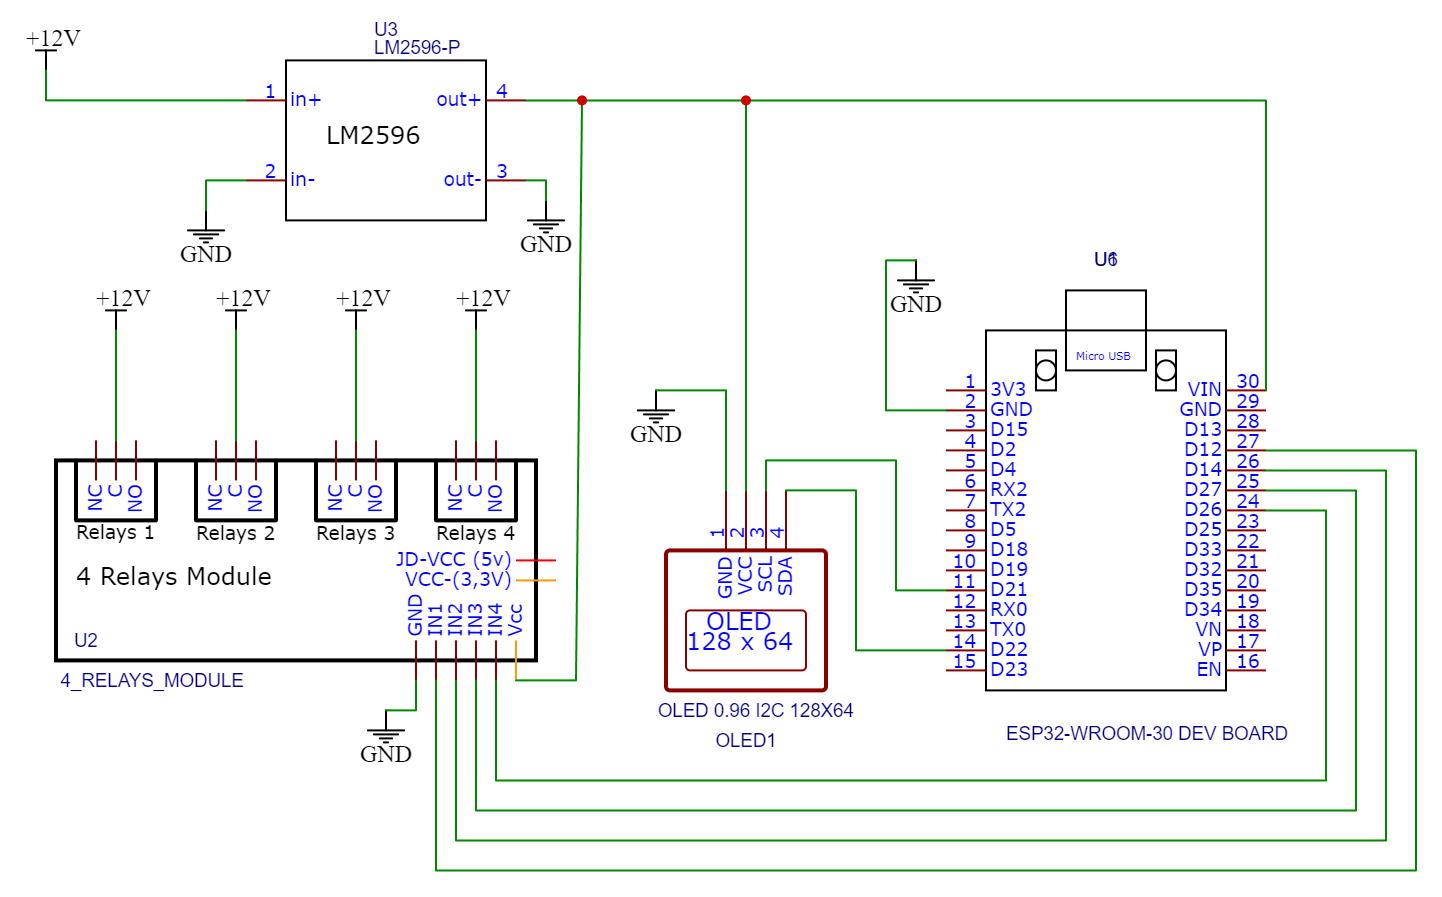
\includegraphics[width=0.9\textwidth]{./Figures/pump_schem.png}
	\caption[Conexión del módulo de control de riego]{Conexión del módulo de control de riego.}
	\label{fig:riegochem}
\end{figure}



\begin{figure}[!h]
     \centering
     \begin{subfigure}[b]{0.45\textwidth}
		\centering
		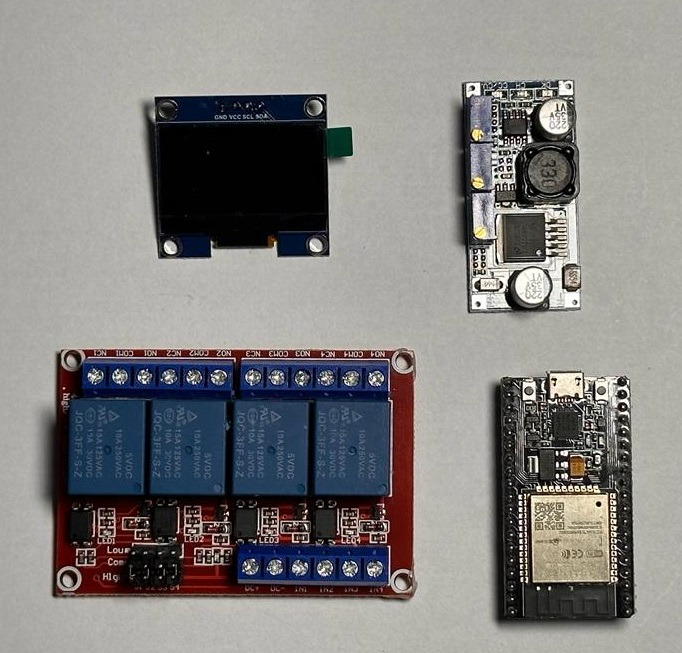
\includegraphics[width=0.8\textwidth]{./Figures/control_riego1.jpg}
		\caption[Detalle de los componentes]{Detalle de los componentes.}
		\label{fig:riego1}
     \end{subfigure}
     \hfill
     \begin{subfigure}[b]{0.45\textwidth}
	\centering
		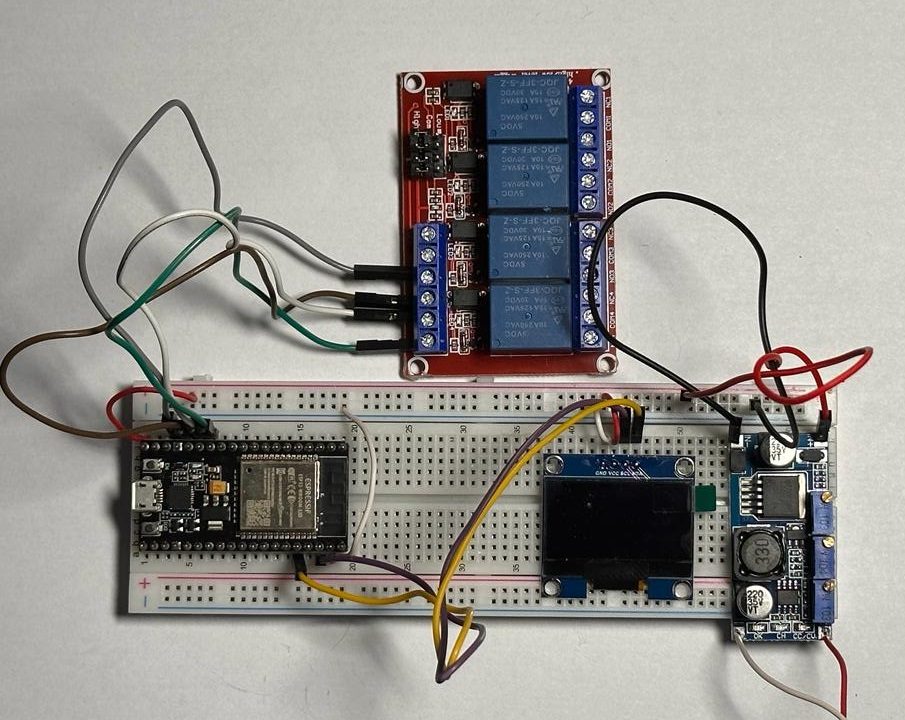
\includegraphics[width=1\textwidth]{./Figures/control_riego2.jpg}
		\caption[Conexionado]{Conexionado.}
		\label{fig:riego2}
     \end{subfigure}
      \begin{subfigure}[b]{0.45\textwidth}
	\centering
		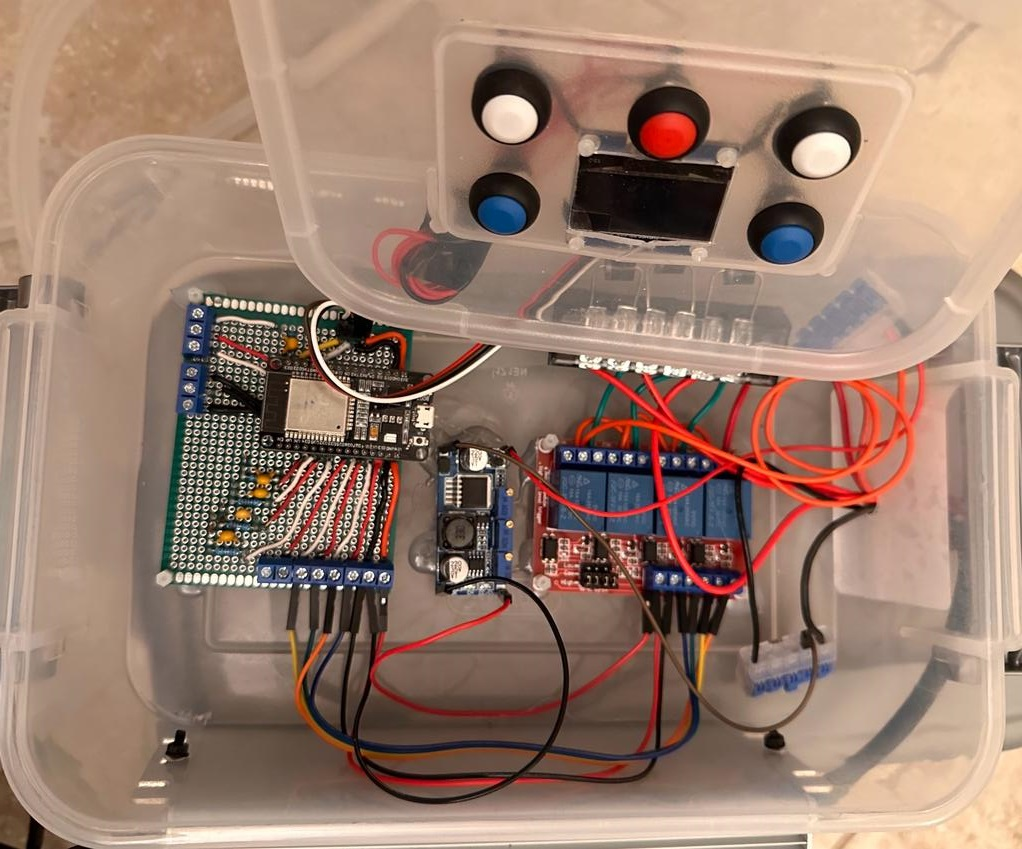
\includegraphics[width=0.8\textwidth]{./Figures/control_riego3.jpg}
		\caption[Conexionado]{Módulo finalizado en su caja protectora.}
		\label{fig:riego3}
     \end{subfigure}	
%			\begin{subfigure}[b]{0.45\textwidth}
%	\centering
%		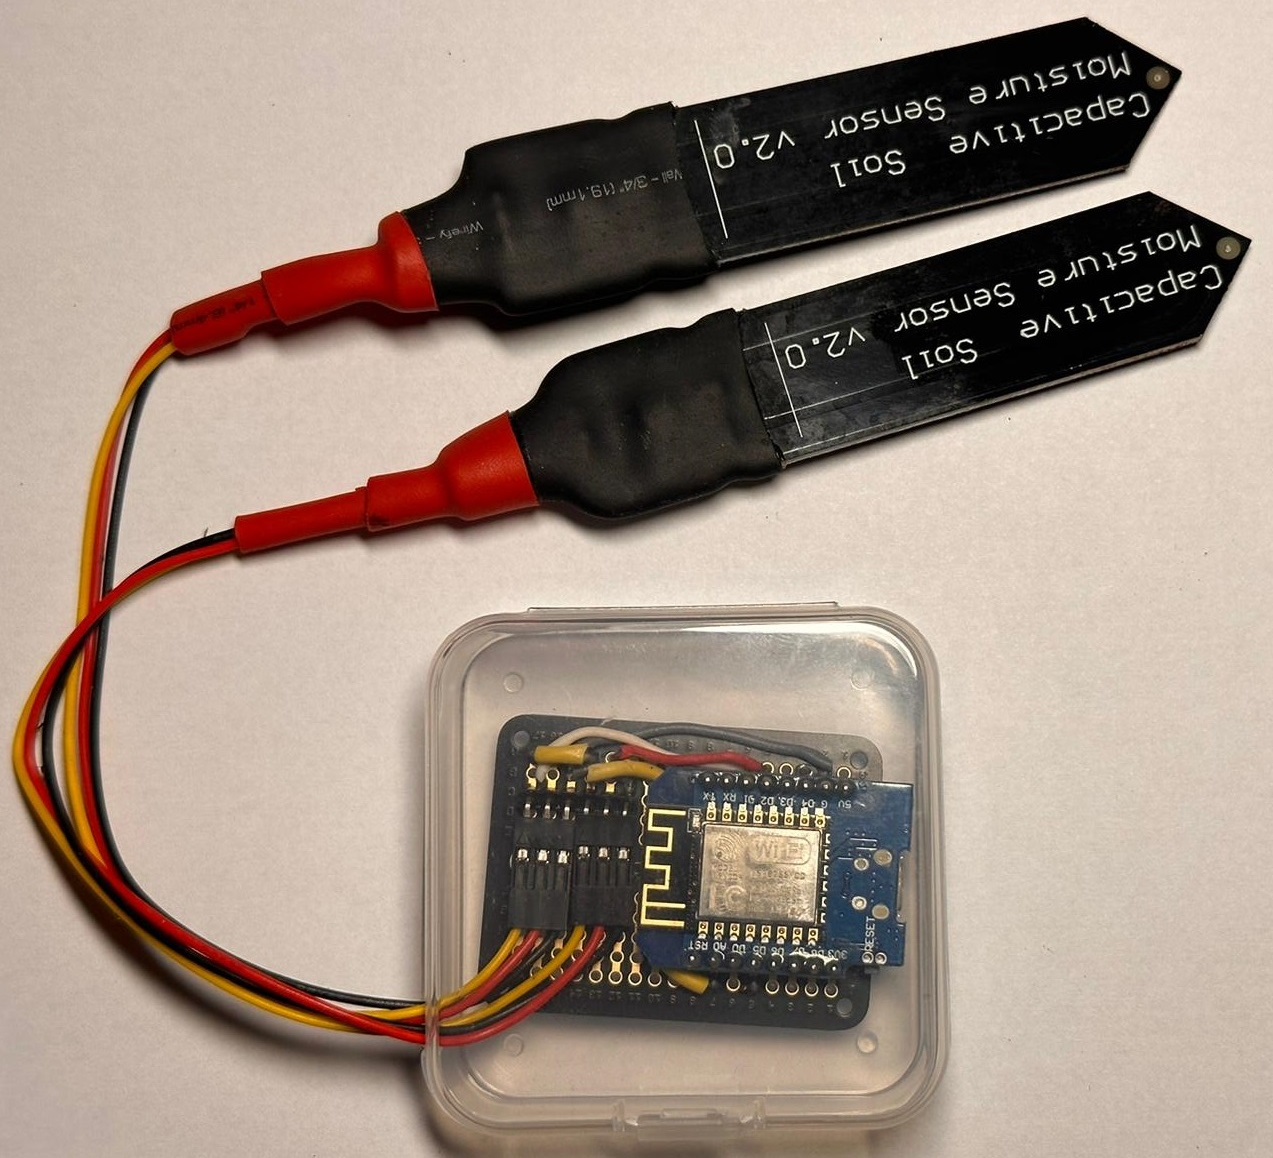
\includegraphics[width=0.60\textwidth]{./Figures/soil3.jpg}
%		\caption[Módulo en su caja protectora]{Módulo en su caja protectora.}
%		\label{fig:soil4}
%     \end{subfigure}
     \hfill
        \caption[Módulo de control de riego]{Módulo de control de riego.}
        \label{fig:riego_control}
\end{figure}


%\begin{figure}[!h]
%	\centering
%	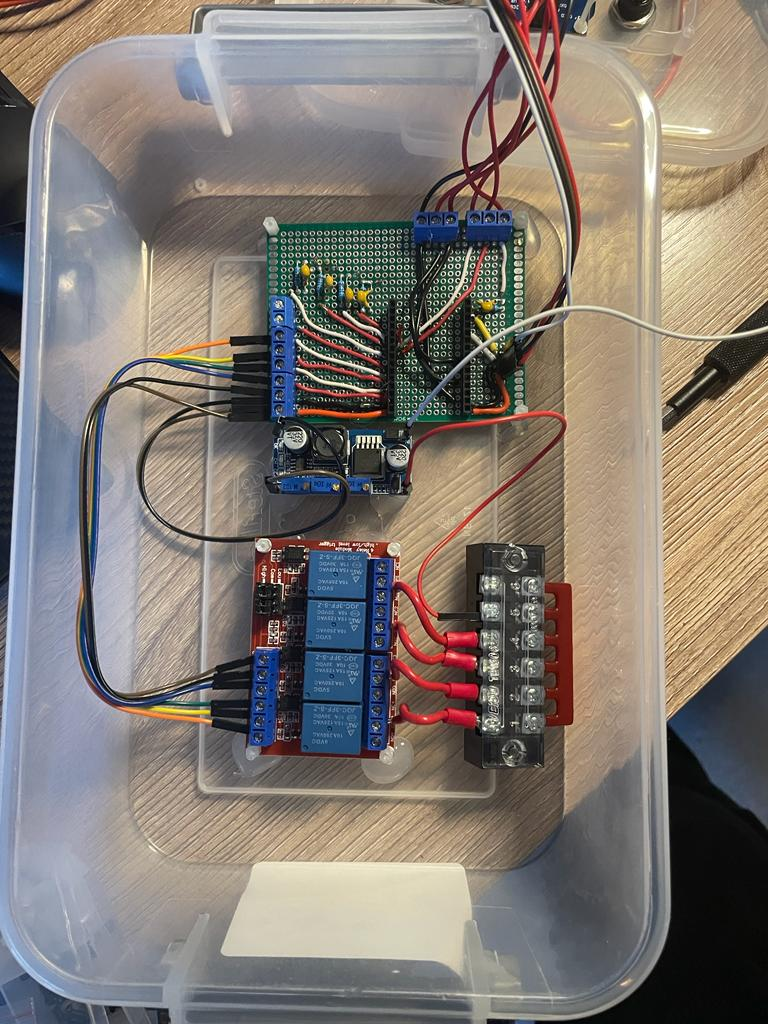
\includegraphics[width=0.5\textwidth]{./Figures/riego1.jpg}
%	\caption[Módulo completo en su caja protectora]{Módulo completo en su caja protectora.}
%	\label{fig:riego_control}
%\end{figure}
 
\pagebreak

\subsection{Módulo sensor de temperatura y humedad}
\label{Módulo sensor de temperatura y humedad}

Está compuesto por un microcontrolador ESP8266, un sensor DHT22 y una pantalla LCD/OLED SSH1106 para visualizar los valores de temperatura y humedad  \textit{in situ} en tiempo real. El esquema de conexión de los componentes se puede ver en la figura \ref{fig:tempschem}.

A diferencia de las sondas de humedad del suelo, el sensor de temperatura y humedad está pensado para instalarse en una ubicación fija 
con acceso a la red eléctrica. Por este motivo no se consideró configurarlo para soportar \textit{deep sleep}.



La construcción del módulo se realizó sobre placa PCB experimental en forma similar a los demás sistemas.
Para proteger los componentes se utilizó una caja de polipropileno transparente. El sensor DHT22 quedó expuesto para medir las condiciones ambientales como muestra la figura \ref{fig:temp_sensor}.


\begin{figure}[!h]
	\centering
	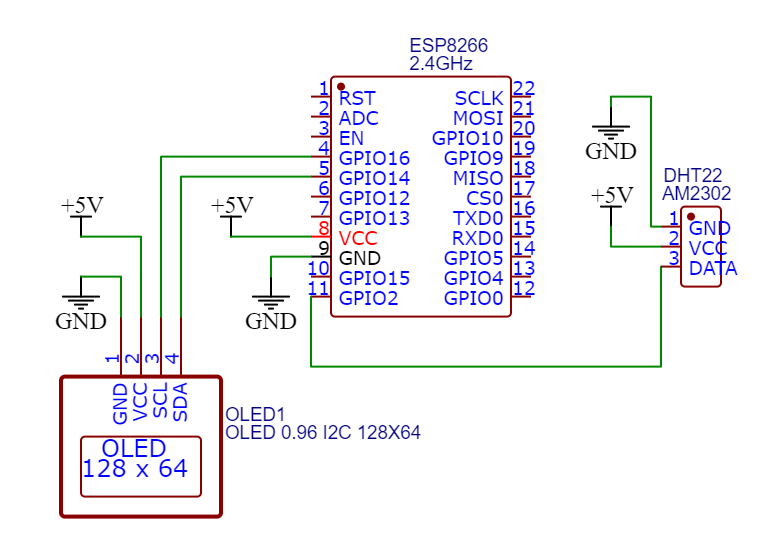
\includegraphics[width=0.7\textwidth]{./Figures/temp_sensor.png}
	\caption[Conexión del sensor de temperatura y humedad]{Conexión del sensor de temperatura y humedad.}
	\label{fig:tempschem}
\end{figure}


\begin{figure}[!h]
	\centering
	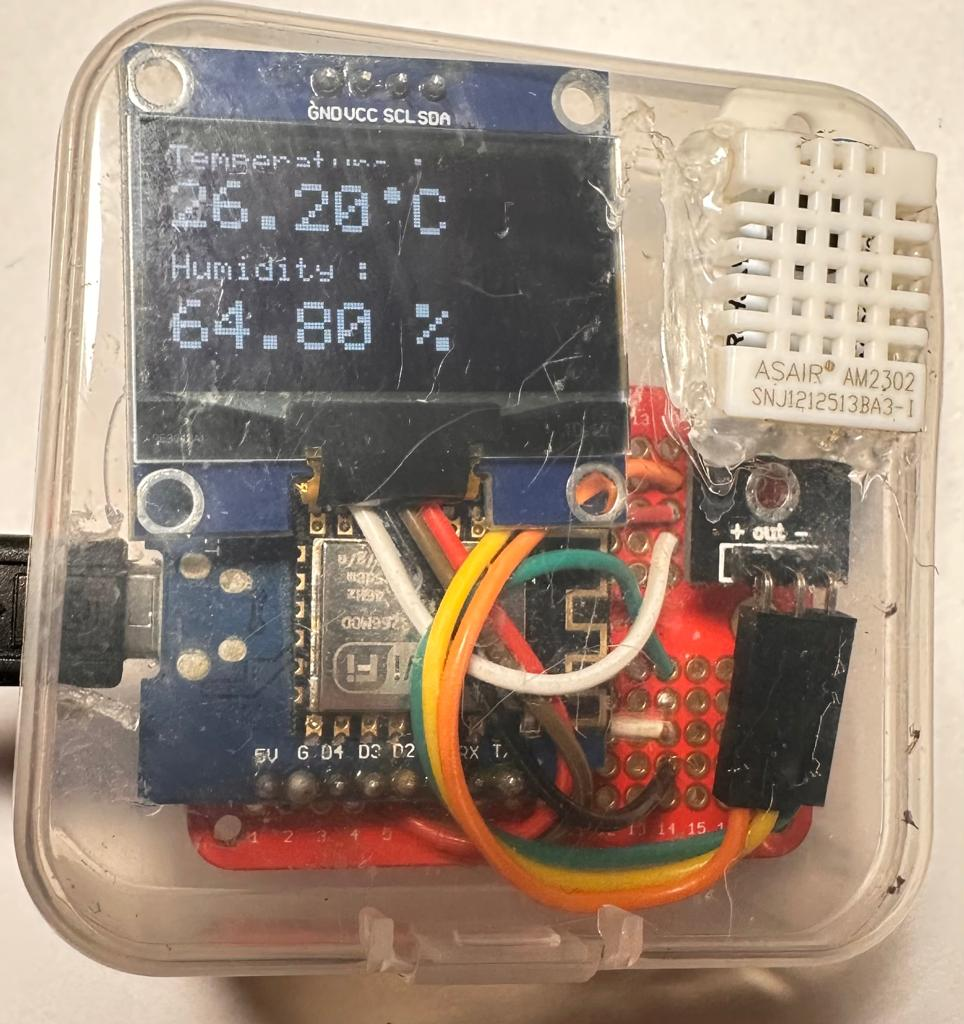
\includegraphics[width=0.5\textwidth]{./Figures/sensor_temp.jpg}
	\caption[Módulo completo en su caja protectora]{Módulo completo en su caja protectora.}
	\label{fig:temp_sensor}
\end{figure}


\subsection{Módulo controlador de clima}
\label{Módulo controlador de clima}

Es el responsable de accionar los ventiladores en el invernadero. Para el diseño se utilizó un chip ESP8266 conectado a un relé de una vía como se muestra en la figura \ref{fig:ventschem}. 

Dado que la salida del microcontrolador es de 3,3 V para el prototipo se seleccionó un relé que pueda ser accionado con ese valor de tensión, para evitar el uso de componentes adicionales tales como convertidores de tensión DC-DC \textit{step up}. 

En la figura \ref{fig:ventcontrol} se ilustra el proceso de construcción del módulo. 



\begin{figure}[!h]
	\centering
	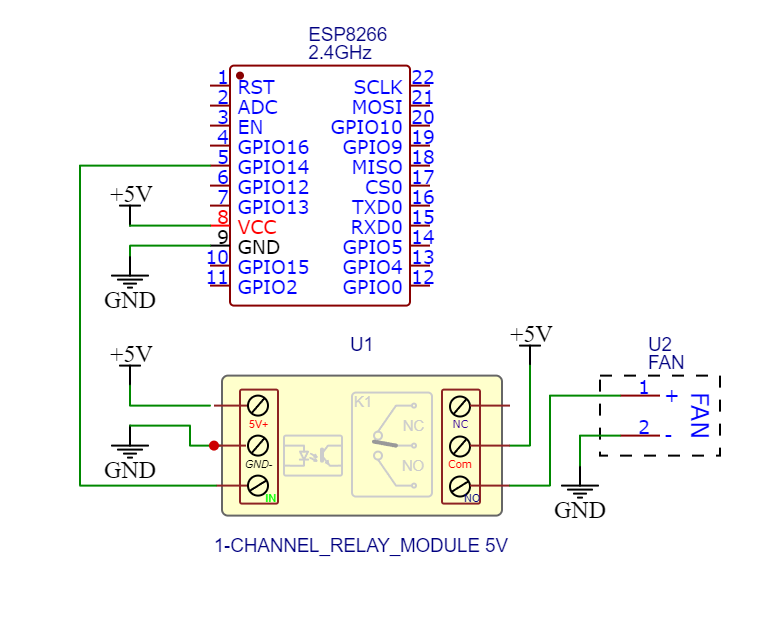
\includegraphics[width=0.7\textwidth]{./Figures/vent_schem.png}
	\caption[Conexión del módulo de control de clima]{Conexión del módulo de control de clima.}
	\label{fig:ventschem}
\end{figure}


\begin{figure}[!htpb]
     \centering
     \begin{subfigure}[b]{0.45\textwidth}
		\centering
		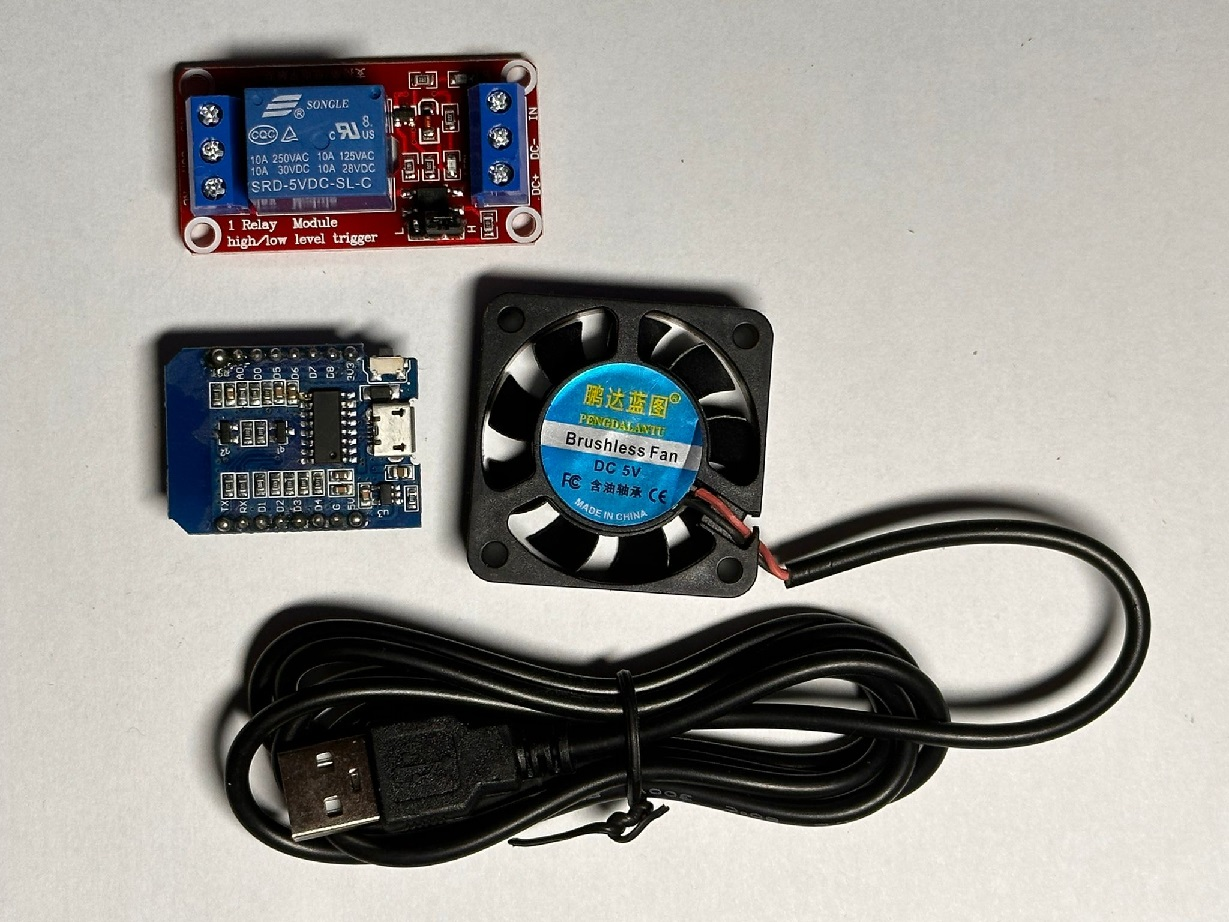
\includegraphics[width=0.80\textwidth]{./Figures/vent_control.jpg}
		\caption{Detalle de los componentes.}
		\label{fig:vent1}
     \end{subfigure}
     \hfill
     \begin{subfigure}[b]{0.45\textwidth}
	\centering
		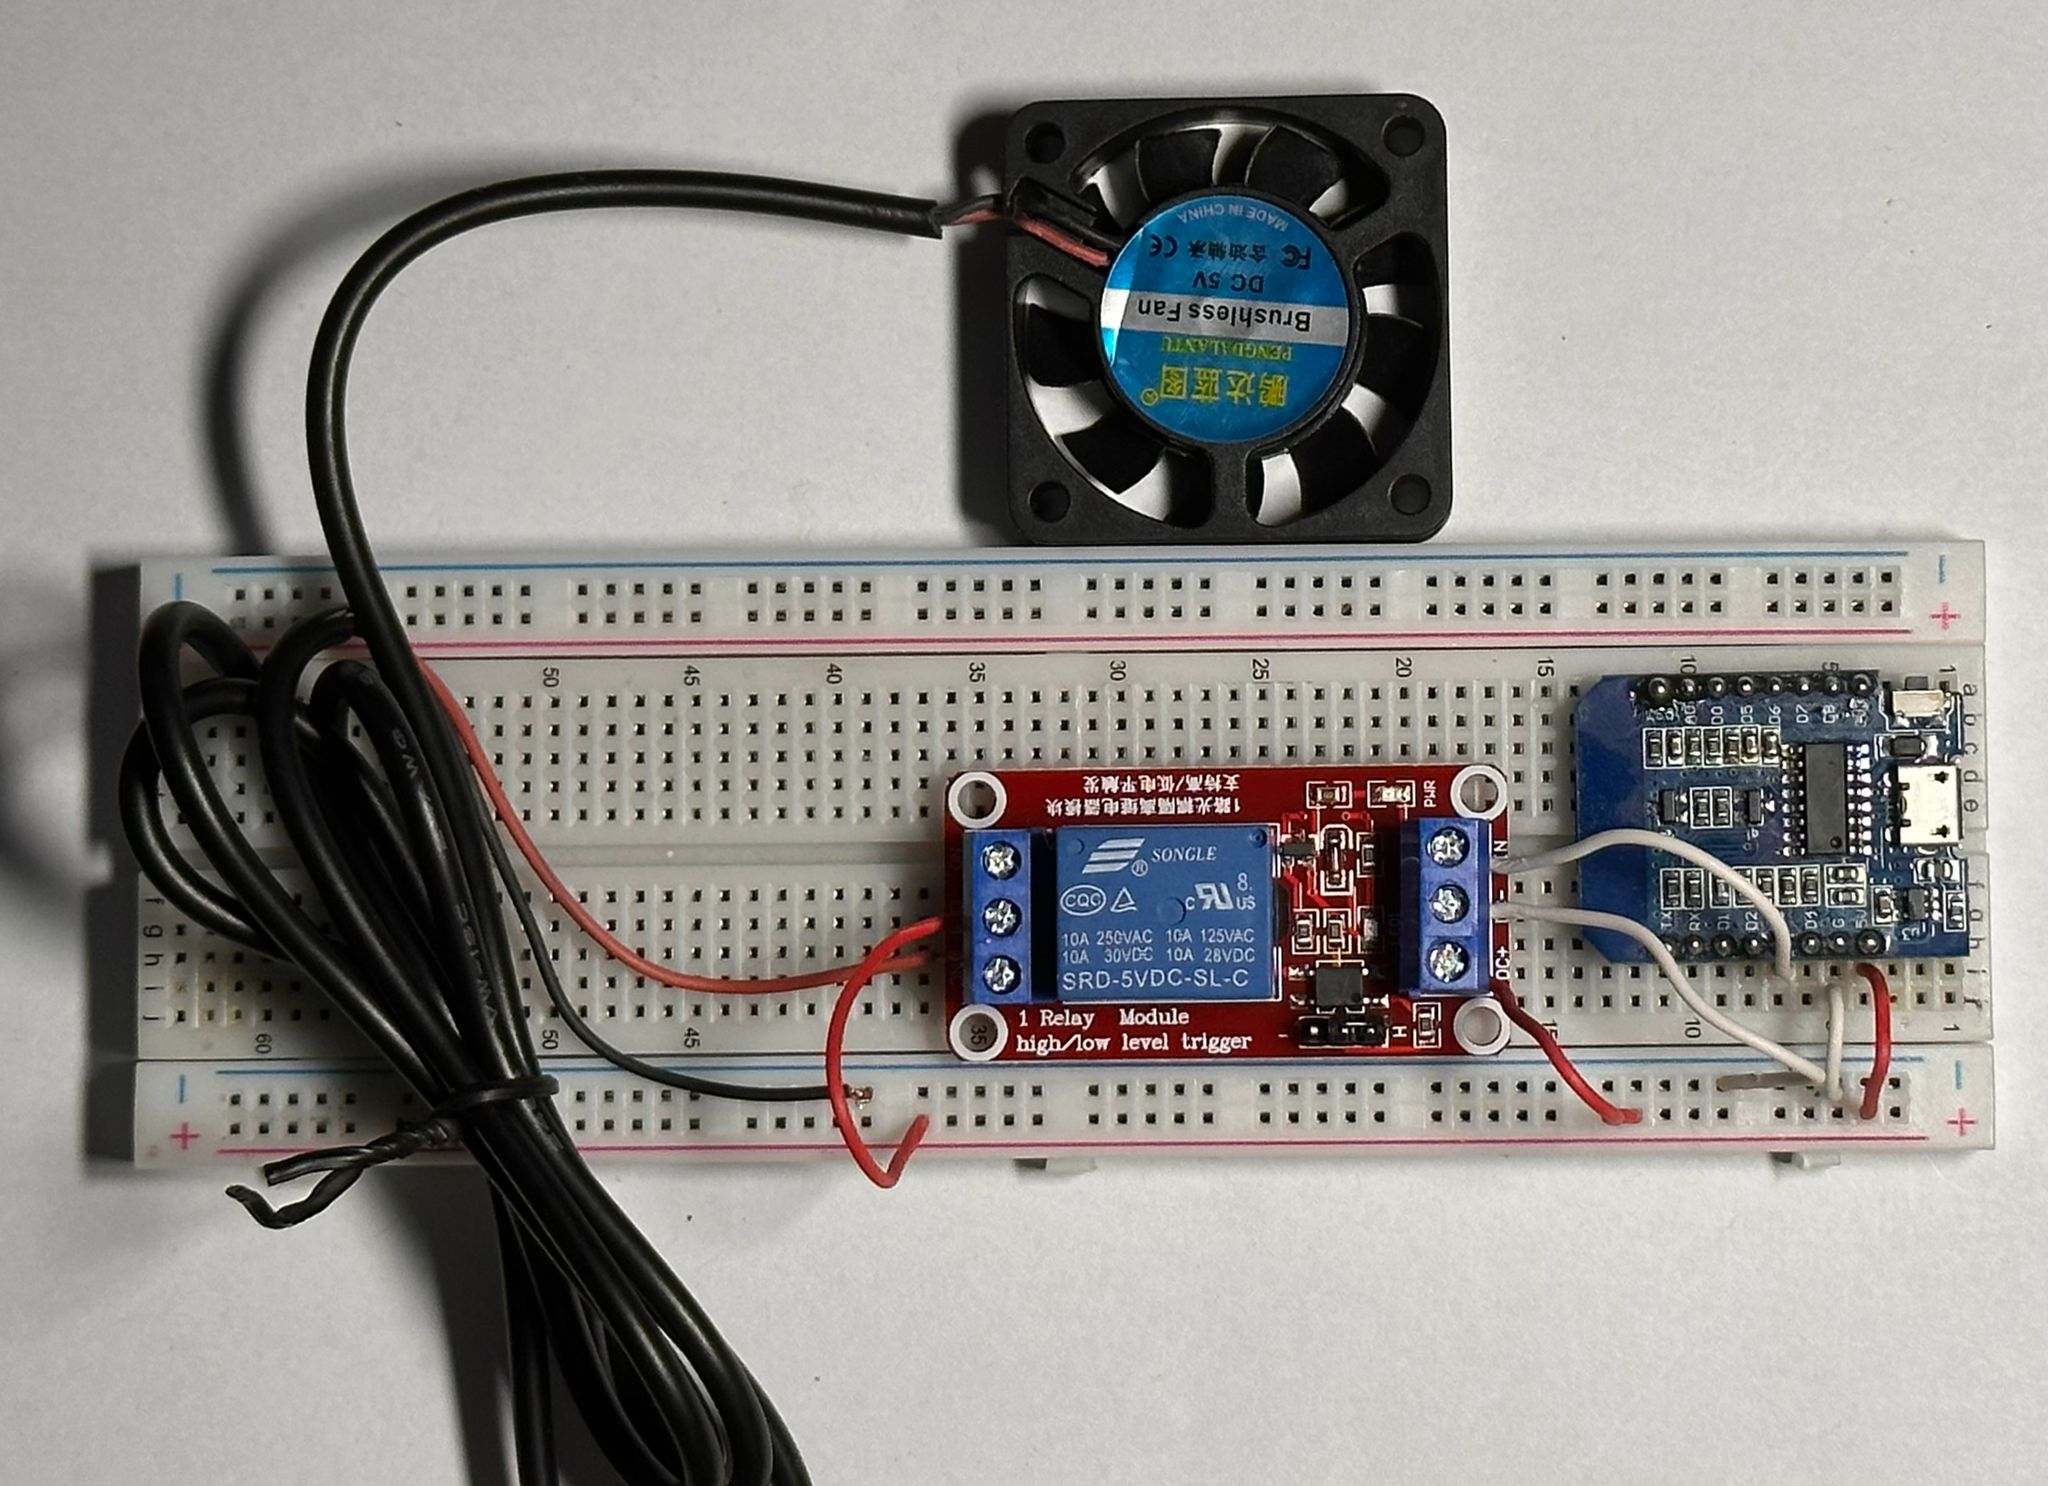
\includegraphics[width=0.80\textwidth]{./Figures/vent_proto.jpg}
		\caption{Conexionado.}
		\label{fig:vent2}
     \end{subfigure}	
	\begin{subfigure}[b]{0.45\textwidth}
		\centering
		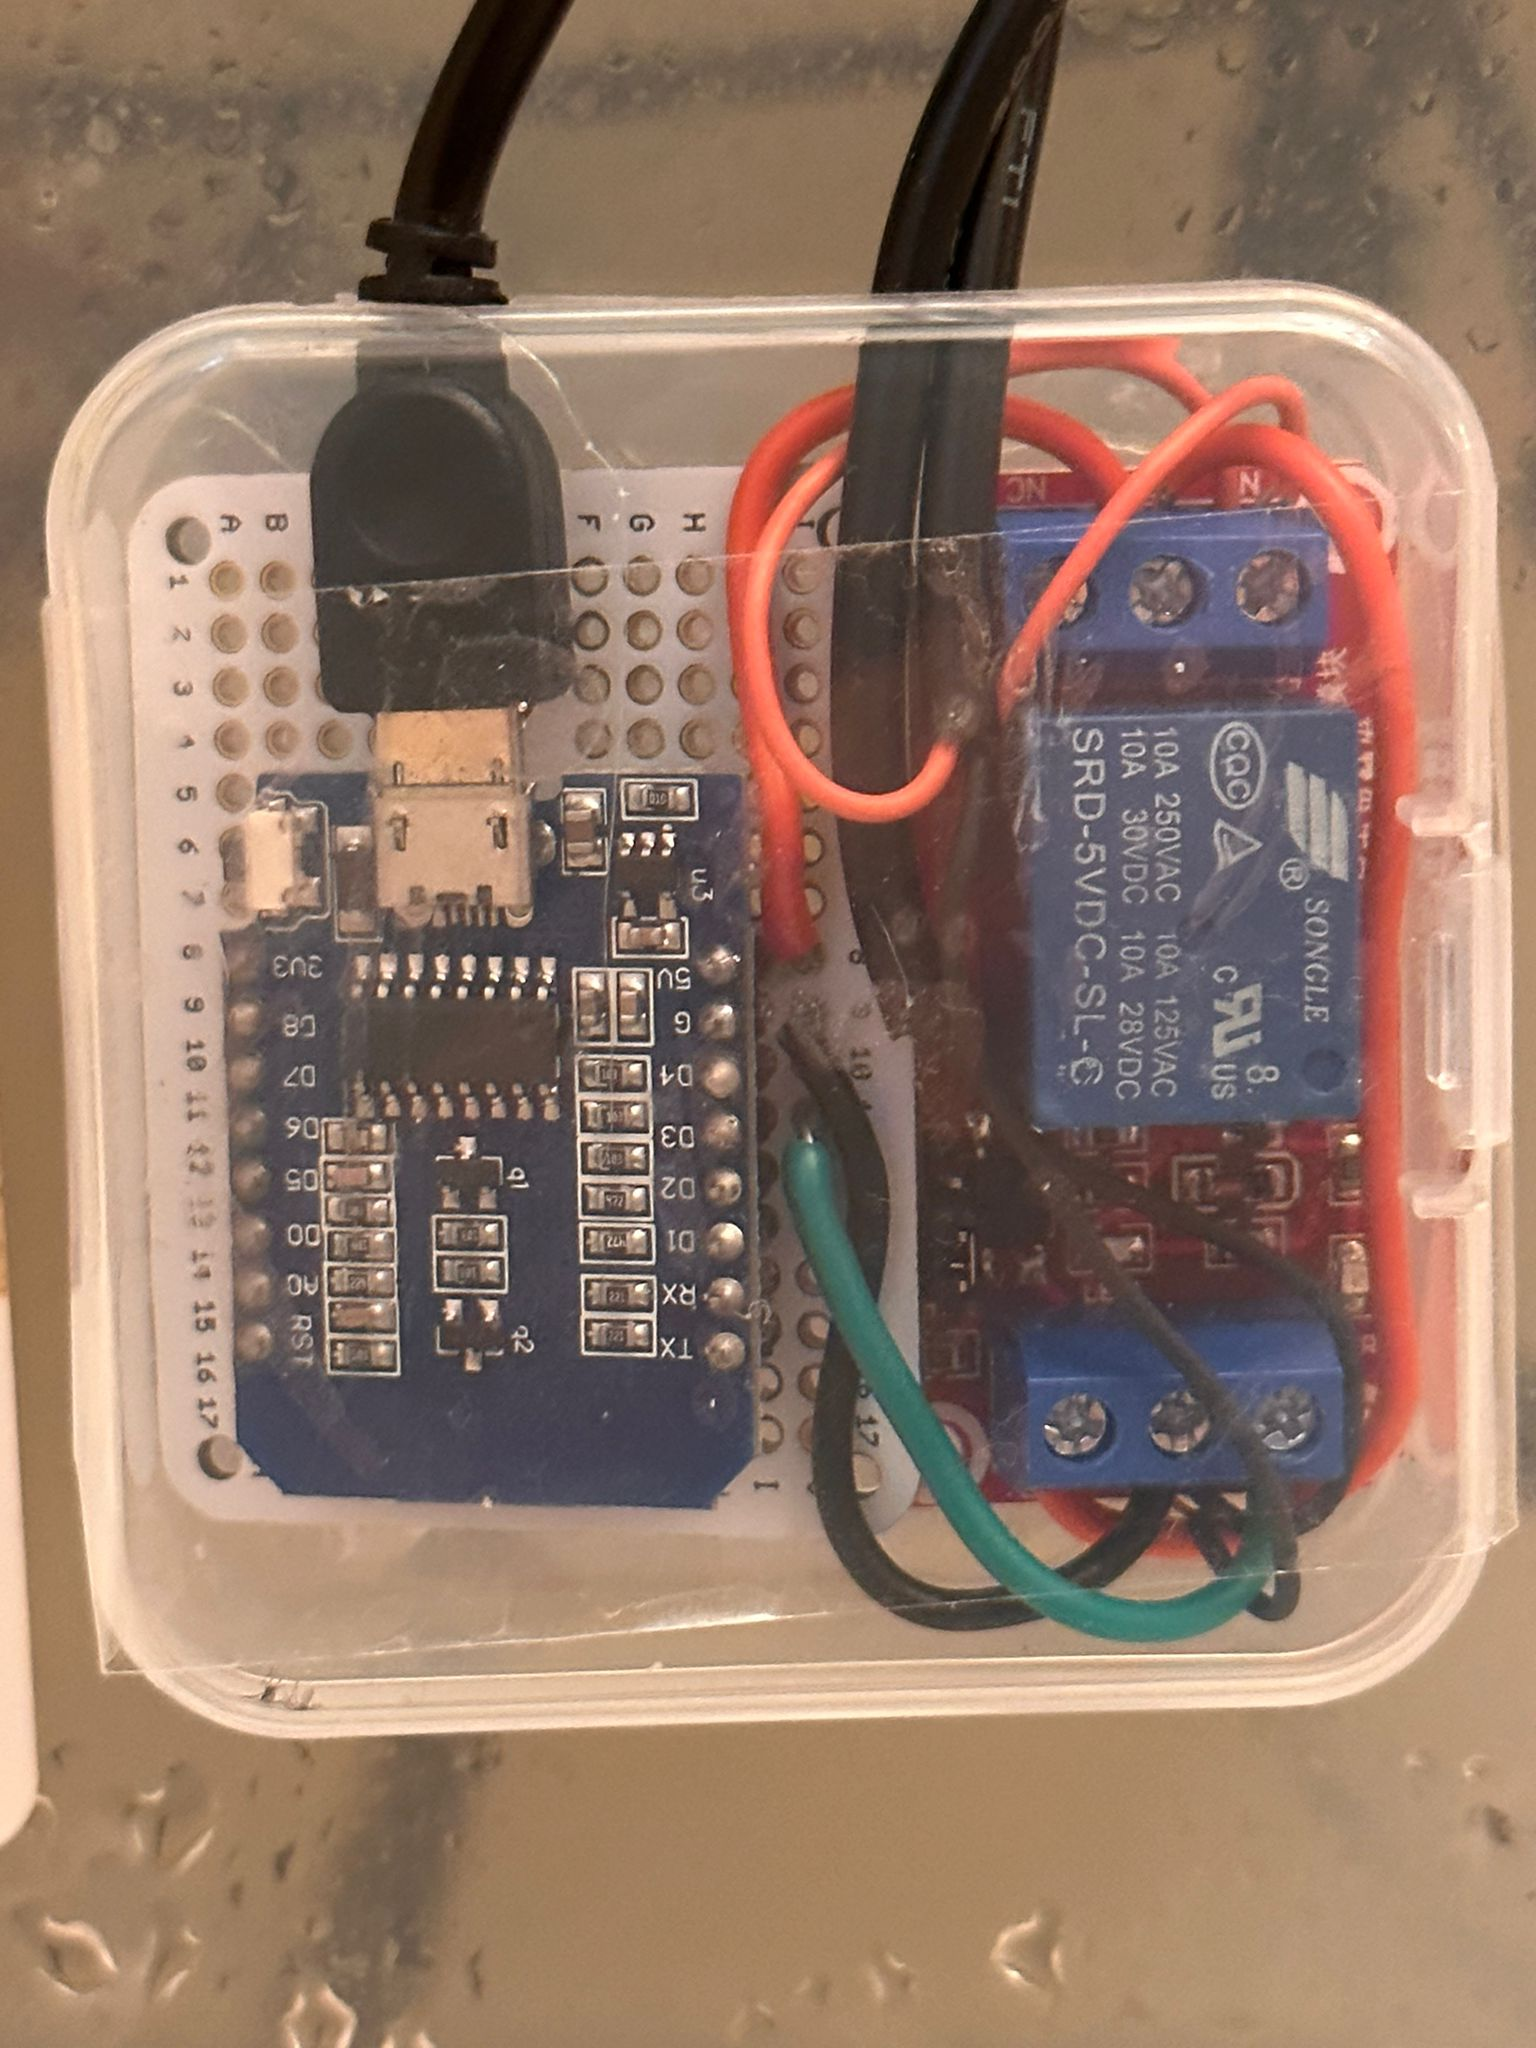
\includegraphics[width=0.60\textwidth]{./Figures/vent_assembled.jpg}
		\caption{Módulo finalizado en su caja protectora.}
		\label{fig:vent3}
     \end{subfigure}
     \hfill
        \caption[Módulo de control del clima]{Módulo de control del clima.}
        \label{fig:ventcontrol}
\end{figure}


\pagebreak

\section{Desarrollo del firmware}
\label{sec:Desarrollo del firmware}

Para la realización del proyecto se optó por desarrollar el firmware de todos los módulos en C++ por medio de la aplicación Arduino IDE. Los criterios utilizados para esta selección se basaron en la baja curva de aprendizaje de la herramienta, la amplia disponibilidad de librerías y ejemplos para el uso de componentes y la vasta comunidad de soporte para entusiastas de IoT existente en Internet.  Estos factores resultaron fundamentales para la elección debido a que el soporte y extensión del sistema quedará a cargo del cliente.

En líneas generales, el firmware de todos los módulos sigue el mismo patrón:

\begin{enumerate}
\item Comienzo: se corresponde al encendido del chip.
\item Setup: Es una función especial que se ejecuta una única vez al inicio del programa y se utiliza para inicializar cualquier variable, configurar los pines de entrada y salida y establecer cualquier comunicación que se precise.

\item Loop : Es una función que se ejecuta continuamente en un bucle que por lo general, solo se interrumpe al apagar al dispositivo. En esta sección se coloca el código principal del firmware.
\end{enumerate}
Adicionalmente, el código puede contener variables, funciones y bibliotecas.


Para facilitar la conexión a la aplicación Thingsboard, se hizo uso de la Arduino Thingsboard SDK \citep{tbsdk}, que provee mecanismos para el manejo de MQTT, RPC y provee la opción de realizar actualizaciones de firmware de forma inalámbrica (OTA de \textit{over the air}). 




\subsection{Firmware de los módulos sensores de humedad del suelo}
\label{Firmware de los módulos sensores de humedad del suelo}

Este es el único módulo que utiliza HTTP para la comunicación con la aplicación central debido a limitaciones en la aplicación Thignsboard, al no permitir configurar los períodos de retención de mensajes en las colas de MQTT para soportar configuraciones prolongadas de  \textit{deep sleep}. 

El proceso de ejecución es similar al resto, con la diferencia que luego del inicio, el programa realiza una llamada HTTP para obtener el tiempo de configuración de hibernación. La lectura de los sensores se realiza a continuación y varia de acuerdo a si es una configuración simple o doble. Esto es debido a que el ESP8266 posee un solo pin de conversión analógica a digital (ADC) al que todos las sondas deberán compartir. Para resolver este problema se procede a conectar la alimentación (VCC) de cada una de las sondas un pin GPIO diferente. De esta manera, al encender o apagar estos pines en forma secuencial, se energiza al sensor correspondiente y se procede a leer el valor en el pin ADC, para finalmente apagarlo y repetir el ciclo para el próximo sensor.

Para que el módulo pueda reportar un valor que represente la humedad del suelo, es necesario realizar una conversión del voltaje leído en el pin ADC. Se decidió seguir el método descripto en \citep{soilcalibration} que consiste en realizar mediciones en suelo seco para luego ir agregando cantidades precisas de agua sobre las que se evalúa la diferencia de potencial observada en cada caso. Del proceso resulta una fórmula lineal que calcula el contenido volumétrico de agua presente en la tierra.

Una vez obtenido el o los valores se los reporta a la aplicación por medio una llamada HTTP POST, luego de lo cual el sensor comienza el período de \textit{deep sleep} por la cantidad de tiempo definida en el atributo leído en primera instancia.

En la figura \ref{fig:flow_soilsensor} se diagrama la ejecución del módulo.


\begin{figure}[!h]
	\centering
	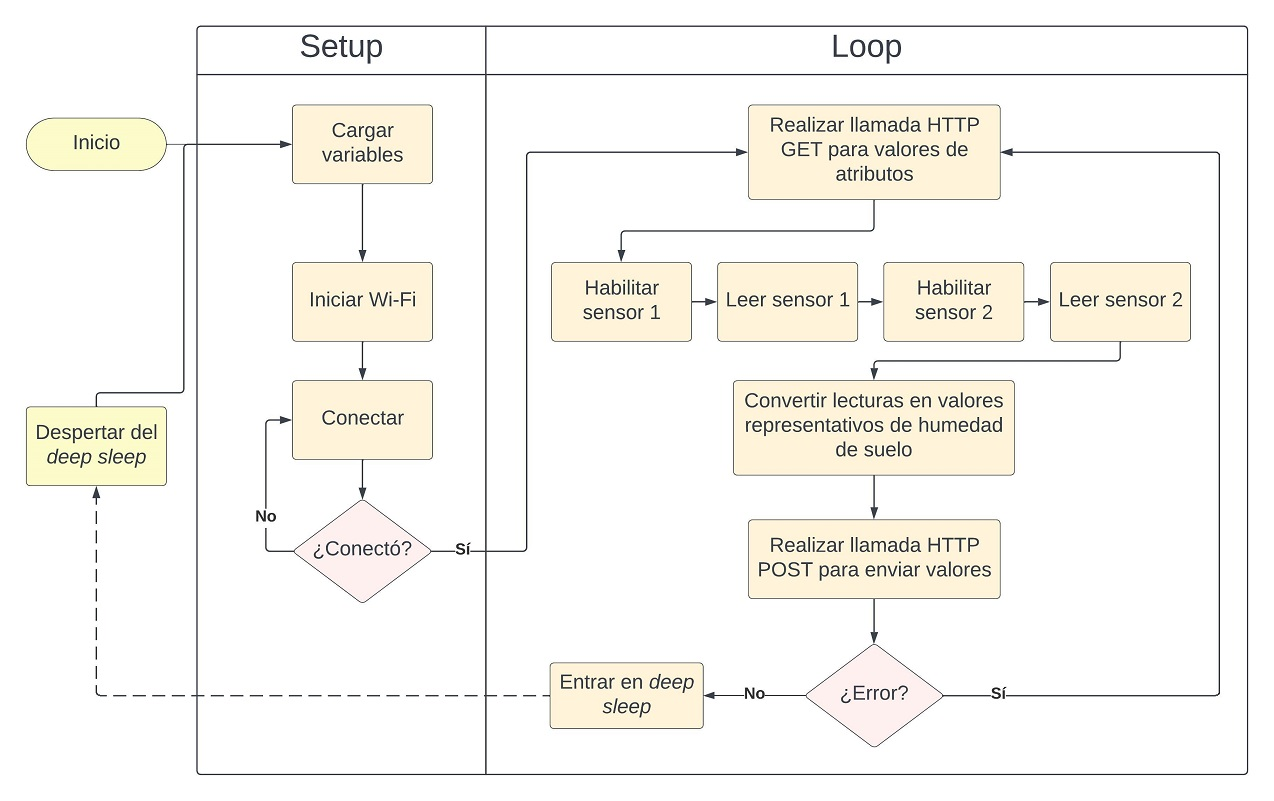
\includegraphics[width=0.9\textwidth]{./Figures/chapter3/FirmwareSoilSensor.jpg}
	\caption[Diagrama de flujo del firmware de los módulos sensores de humedad del suelo]{Diagrama de flujo del firmware de los módulos sensores de humedad del suelo.}
	\label{fig:flow_soilsensor}
\end{figure}


\pagebreak
\subsection{Firmware del módulo controlador del riego}
\label{Firmware del módulo controlador del riego}

Este es el módulo de mayor complejidad lo que puede verse reflejado en las figuras \ref{fig:flow_riegocontrol}, \ref{fig:flow_valvecontrol}  y \ref{fig:flow_bombacontrol}.

La ejecución se inicializa con el proceso estándar de carga de variables, entre las que se incluye un valor por defecto para la duración del riego, y el estado de la bomba y cada válvula presente. Luego de la conexión a la red Wi-Fi, el programa se registra a la aplicación y se subscribe a los \textit{getter topics} y a los  \textit{setter topics}, que se corresponden a los canales para reportar los estados a la aplicación o recibir comandos para prender o apagar dispositivos respectivamente.

En el caso de recibir un mensaje para informar el estado de los pines de GPIO, asociados con las válvulas o la bomba, o de la variable de duración de riego, el código reporta sobre el \textit{topic} de respuesta el estado requerid. En cambio, si el mensaje recibido para realizar un cambio, puede suceder una de las siguientes situaciones: es para comenzar el riego, el programa realiza una serie de verificaciones para asegurar la integridad de la bomba y cañerías del sistema de riego:
\begin{itemize}
\item Pedido de reconfigurar el tiempo de riego: el código actualiza la variable y retorna la comienzo del bucle.

\item Pedido de apertura o cierre de válvula:
    \begin{itemize}
    \item Apertura: Se procede a abrir la válvula seleccionada y se comprueba si la bomba esta en estado de pedido de encendido (bomba lista), en cuyo caso se ordena el encendido de la bomba.
    \item Cierre: se realiza una comprobación si hay otras válvulas abiertas, de ser así se procede con el cierre. En caso de ser la última, se ordena el apagado de la bomba y por último se procede al cierre de válvula.
    
    \end{itemize}

\item Pedido de prendido o apagado de la bomba:
    \begin{itemize}
    \item Prendido: En el caso de haber una válvula abierta, se procede a encender la bomba por el tiempo que marque la variable de duración de riego, luego de lo cual se procede al apagado de la bomba y cierre de las válvulas, en ese orden. De no haber válvulas abiertas, se configura la variable de bomba lista en positivo, indicando que el riego fue pedido pero aún no están dadas las condiciones.
    \item Apagado: En el caso de pedir una interrupción en el riego, se ordena el apagado de la bomba y el cierre de las válvula.
    
    \end{itemize}



\end{itemize}


\begin{figure}[!h]
	\centering
	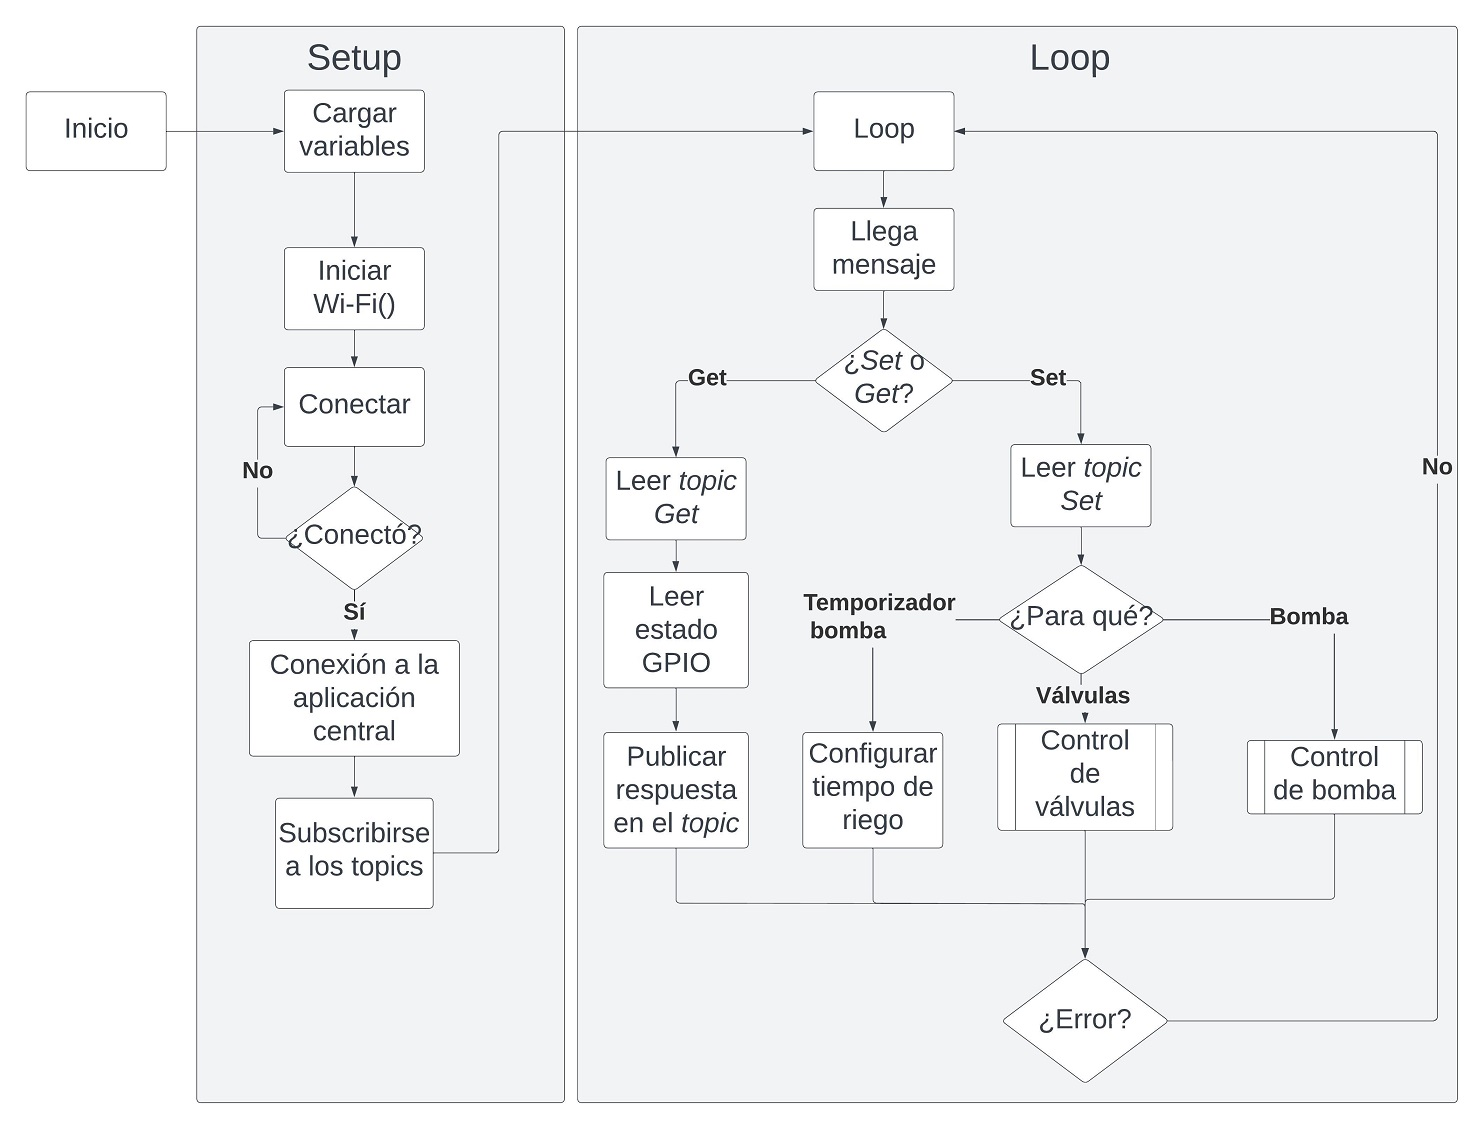
\includegraphics[width=0.9\textwidth]{./Figures/chapter3/FirmwareRiegoControl.jpg}
	\caption[Diagrama de flujo del firmware del módulo de control de riego]{Diagrama de flujo del firmware del módulo de control de riego.}
	\label{fig:flow_riegocontrol}
\end{figure}

\begin{figure}[!h]
	\centering
	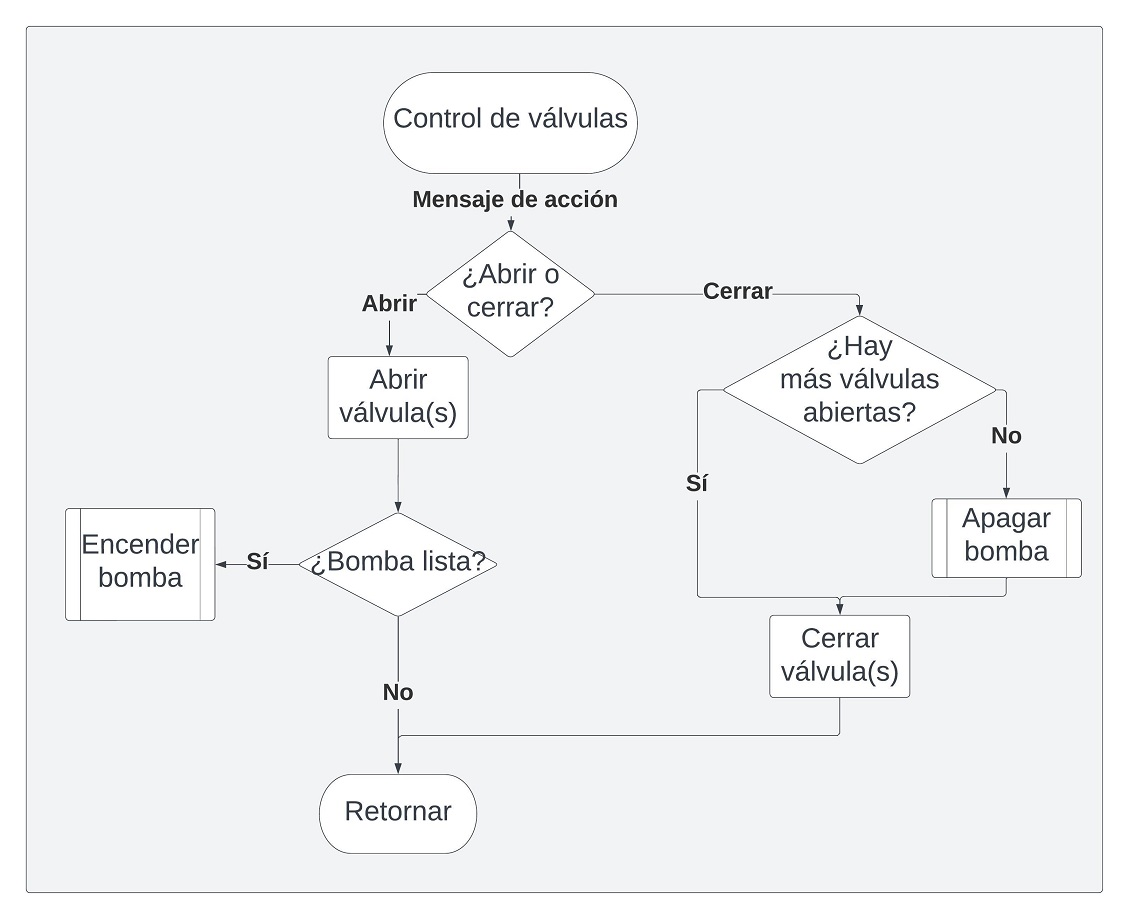
\includegraphics[width=0.7\textwidth]{./Figures/chapter3/FirmwareValveControl.jpg}
	\caption[Diagrama de flujo del firmware del módulo de control de riego - Control de válvulas]{Diagrama de flujo del firmware del módulo de control de riego - Control de válvulas.}
	\label{fig:flow_valvecontrol}
\end{figure}

\begin{figure}[!h]
	\centering
	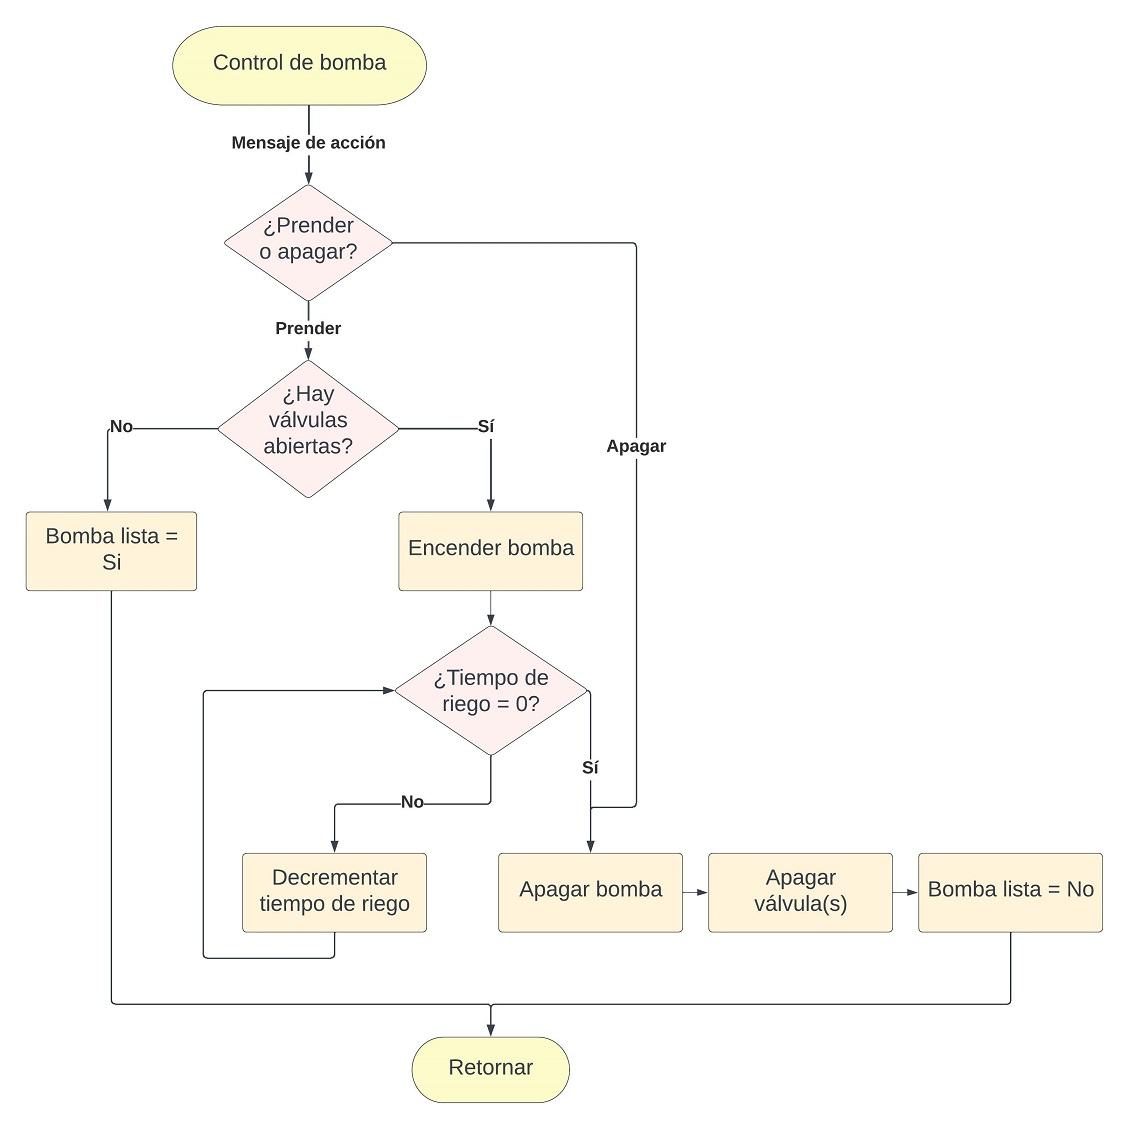
\includegraphics[width=0.7\textwidth]{./Figures/chapter3/FirmwarePumpControl.jpg}
	\caption[Diagrama de flujo del firmware del módulo de control de riego - Control de bomba]{Diagrama de flujo del firmware del módulo de control de riego - Control de bomba.}
	\label{fig:flow_bombacontrol}
\end{figure}







\pagebreak
\subsection{Firmware de los módulos sensores de temperatura y humedad}
\label{Firmware de los módulos sensores de de temperatura y humedad}

Se encarga de obtener las medidas de temperatura y humedad y reportarlas a la aplicación al mismo tiempo que imprime los valores en la pantalla LCD. Para reducir la cantidad de mensajes enviados, se incorpora un contador que indica cuántas iteraciones del ciclo son necesarias por cada envío de datos. Esto no se contempla para el reporte en la pantalla.


\begin{figure}[!h]
	\centering
	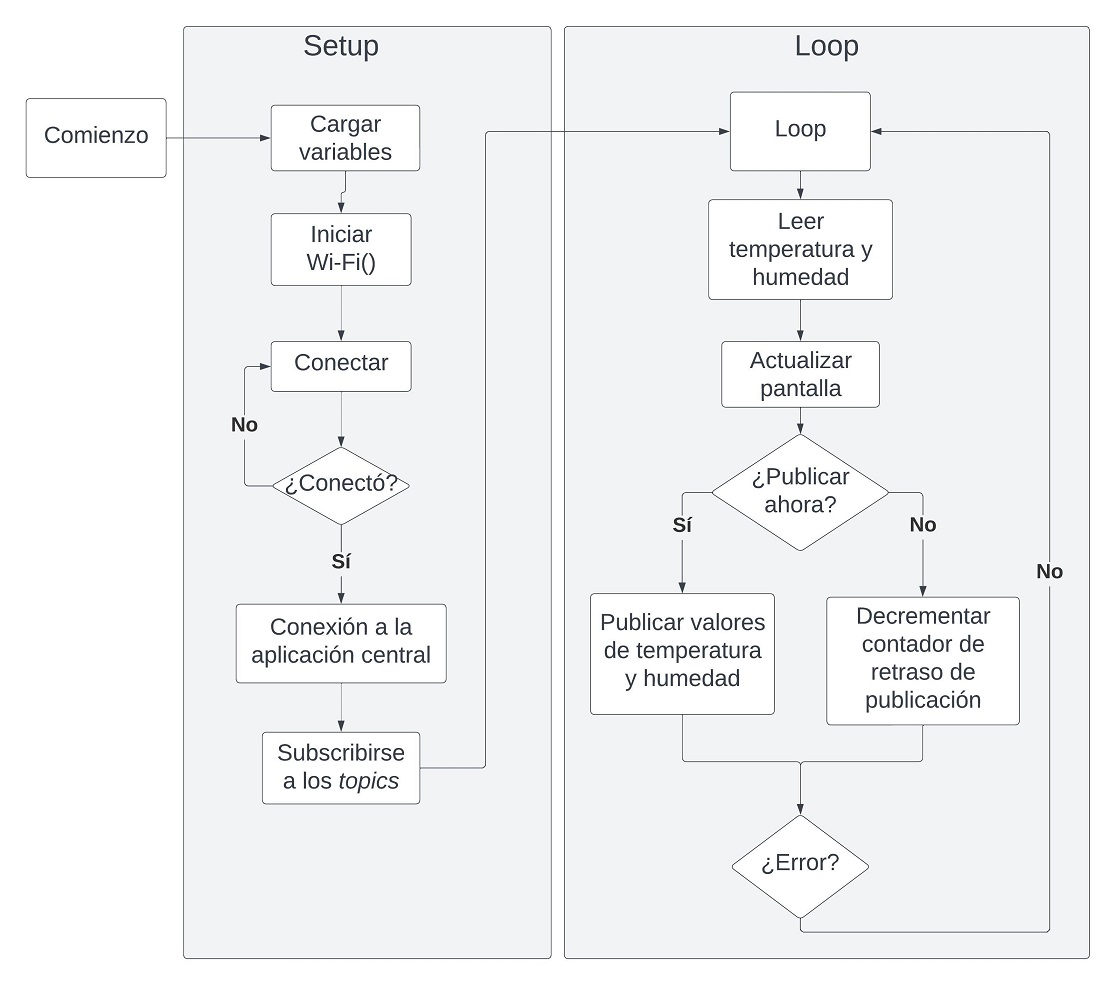
\includegraphics[width=0.8\textwidth]{./Figures/chapter3/FirmwareTempSensor.jpg}
	\caption[Diagrama de flujo del firmware del módulos sensores de temperatura y humedad]{Diagrama de flujo del firmware del módulos sensores de temperatura y humedad.}
	\label{fig:flow_tempsensor}
\end{figure}

\pagebreak
\subsection{Firmware del módulo de control de clima}
\label{Firmware del módulo de control de clima}

Es el que se encarga del encendido y apagado de los ventiladores para el control de clima.
Luego de la comienzo, el programa se conecta a la red, se subscribe en los \textit{topics} correspondientes, y queda a la espera de los mensajes. En el caso de recibir un pedido de reporte, responde con el estado del pin GPIO asociado con el ventilador. Si recibe un pedido de prendido o apagado, realiza la acción correspondiente y retorna al inicio del bucle.


\begin{figure}[!h]
	\centering
	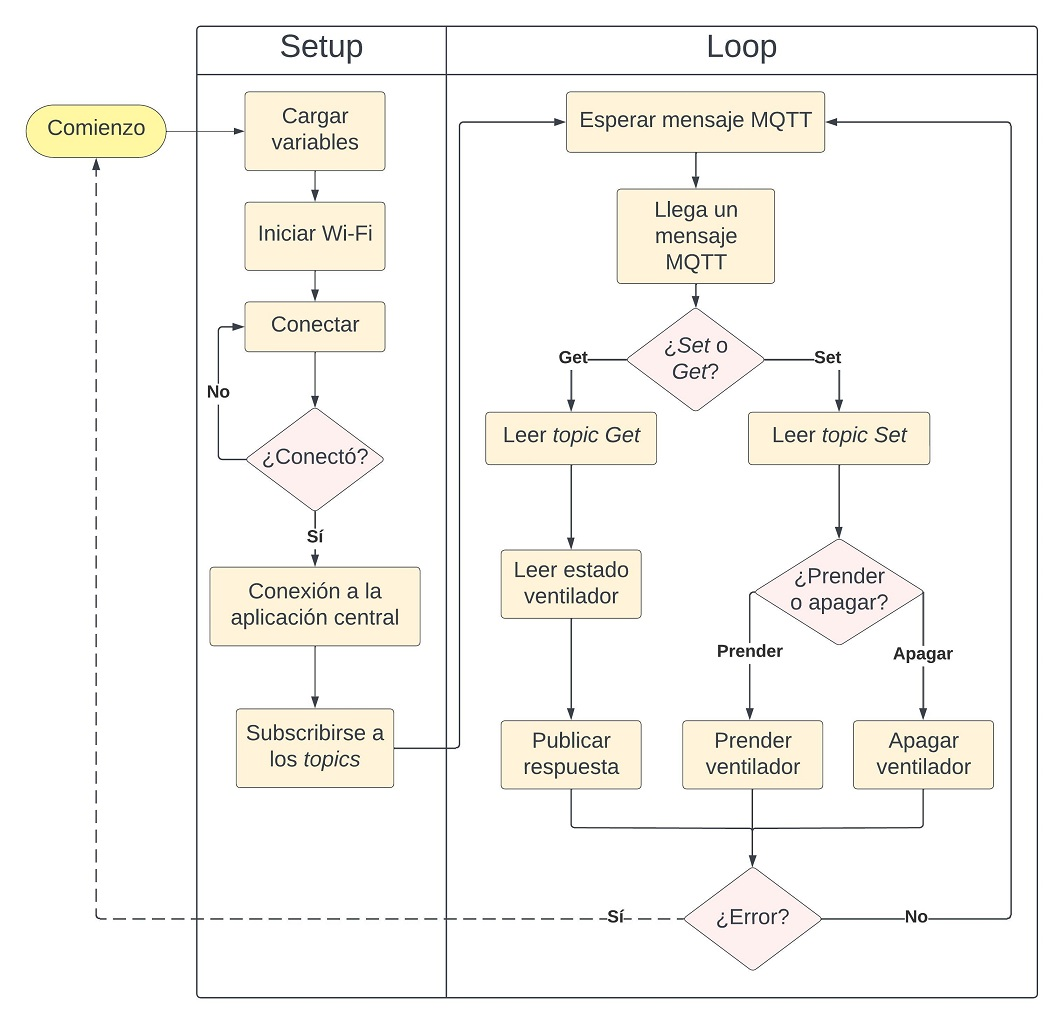
\includegraphics[width=0.8\textwidth]{./Figures/chapter3/FirmwareVentControl.jpg}
	\caption[Diagrama de flujo del firmware del módulo de control de clima]{Diagrama de flujo del firmware del módulo de control de clima.}
	\label{fig:flow_climacontrol}
\end{figure}










\pagebreak
\section{Selección y configuración del software}
\label{sec:Selección y configuración del software}

\textcolor{gray}{A desarrollar: en esta sección explicaré los criterios de selección y configuración del software central como así también el diseño de la interfaz de acceso remoto vía Telegram. }

\section{Ciberseguridad del sistema}
\label{sec:Ciberseguridad del sistema}
\textcolor{gray}{A desarrollar: en esta sección explicaré el uso de TLS en las comunicaciones, las limitaciones encontradas y los riesgos residuales. }

